\documentclass[a4paper]{scrartcl}

\usepackage[ngerman]{babel}
\usepackage[utf8]{inputenc}   % Umlaute etc. verwenden
\usepackage[final]{graphicx}    % Grafiken einbinden
\usepackage{url}
\usepackage{float}
\usepackage{framed}
\usepackage{wrapfig}
\parindent 0pt
\usepackage[onehalfspacing]{setspace}
\usepackage{enumerate}

% direkt PDF generieren
\usepackage[pdftex,
    pdftitle={SiLift - Benutzerhandbuch Entwickler},
	pdfauthor={}]{hyperref}
    
% Bis zu welcher Tiefe nummerieren?
\setcounter{secnumdepth}{3}


\begin{document}

% Der Titel der Seminararbeit, sowie der Autor
\title{SiLift - Benutzerhandbuch für Entwickler}
\author{Universität Siegen - Praktische Informatik}

%\date{\today}

\maketitle

%*************************************************************************
%\section{Abstract}
%*************************************************************************
%\begin{abstract}

%\end{abstract}

\newpage

%INHALTSVERZEICHNIS
\tableofcontents
\newpage

%*************************************************************************
\section{Einleitung}
%*************************************************************************

\textit{SiLift} ist ein \textit{Eclipse}-basiertes Framework mit dessen Hilfe sich Differenzen von \textit{EMF-Modellen} \textit{semantisch liften} lassen.\\
Generell werden dabei alle \textit{EMF}-basierten Modellierungssprachen unterstützt, sofern die ent\-sprech\-en\-den \textit{Editier\-regeln} implementiert bzw. aus diesen \textit{Er\-ken\-nungs\-re\-geln} abgeleitet wurden.
Dieses Benutzerhandbuch umfasst neben einer Installationsanleitung einen Einblick in die SiLift-Architektur sowie ein\-führ\-en\-des Tutorial, in dem Sie anhand eines kleinen \textit{Metamodells} lernen mit Hilfe von \textit{EMF-Henshin} Editierregeln zu erstellen um danach aus diesen die Erkennungsregeln abzuleiten.


%*************************************************************************
\section{Voraussetzung und Installation}
%*************************************************************************

SiLift ist als \textit{Eclipse-Feature} unter folgender \textit{Update-Site} erhältlich:\\ \url{http://pi.informatik.uni-siegen.de/Projekte/SiLift/updatesite}.\\


\textbf{Hinweis:} Vergewissern Sie sich, ob ihr Eclipse die notwendigen Voraussetzungen erfüllt. 
Eine Liste der benötigten Plugins ist unter \url{http://pi.informatik.uni-siegen.de/Projekte/SiLift/download.php} zu finden.
Bitte beachten Sie dabei die entsprechenden Hinweise zu den jeweiligen Versionen.\\


Sofern alle Voraussetzungen erfüllt sind, kann SiLift wie gewohnt über den Menüpunkt \texttt{Help} $\triangleright$ \texttt{Install New Software...} installiert werden (vgl. Abb. \ref{eclipse_install_new_software}).

\begin{figure}[H]
\centering
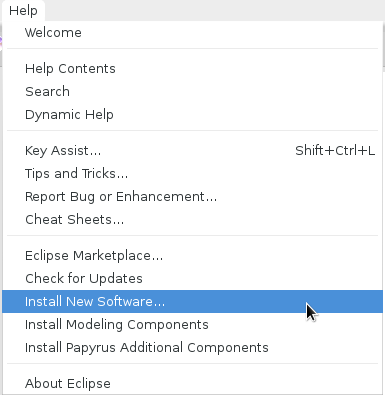
\includegraphics[width=0.25\textwidth]{graphics/eclipse-install_new_software.png}
\caption{Eclipse: Install New Software...}
\label{eclipse_install_new_software}
\end{figure}

Es sollten Ihnen vier Kategorien angezeigt werden (vgl. Abb. \ref{silift_update_site}). 

\begin{figure}[H]
\centering
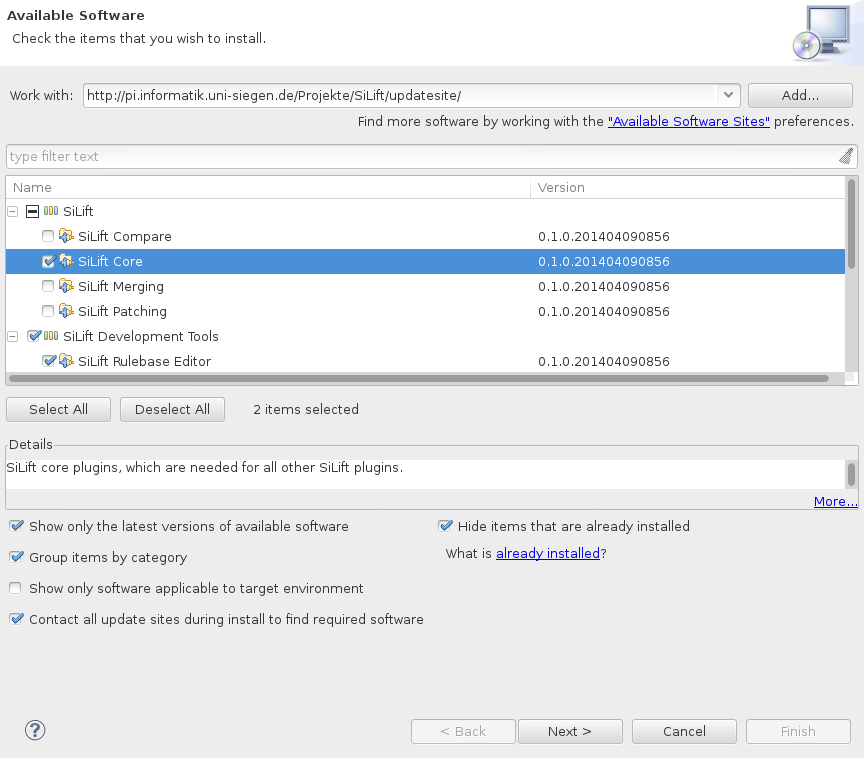
\includegraphics[width=0.6\textwidth]{graphics/eclipse-install_silift.png}
\caption{SiLift Update Site}
\label{silift_update_site}
\end{figure}

Für die folgenden Tutorials benötigen das Feature \texttt{SiLift Core} aus der Kategorie \texttt{SiLift} und das Feature \texttt{SiLift Rule Base Editor} aus der Kategorie \texttt{SiLift Development Tools}. Danach klicken Sie auf \texttt{Next} und folgen dem Installationsassistenten.\\

%*************************************************************************
\section{SiLift-Architektur}\label{silift_architecture}
%*************************************************************************
Mit SiLift können Differenzen von \textit{EMF-basierten} Modellen, d.h. Modelle die auf dem \textit{Ecore-Metamodell} basieren, semantisch geliftet werden. Basierend auf einer gelifteten Differenz lassen sich \textit{Patches} bilden, sowie Modelle mischen.\\
Für \textit{domainspezifische} Modellierungssprachen bedeutet das, dass deren Metamodell (vgl. \ref{subsec:metamodel}) zuerst in ein entsprechendes \textit{Ecore-Modell} übertragen, sowie ein entsprechender \textit{Matcher} (vgl. \ref{sec:own_matching_engine}) und \textit{Technical Difference Builder} (vgl. \ref{sec:TechnicalDifferenceBuilder}) bereit gestellt werden müssen, bevor Editierregeln implementiert und Erkennungsregeln abgeleitet werden können.\\
Dieser Abschnitt führt die \textit{SiLift-Pipline} ein und dient als Grundlage der folgenden Abschnitte.


\begin{figure}[H]
\centering
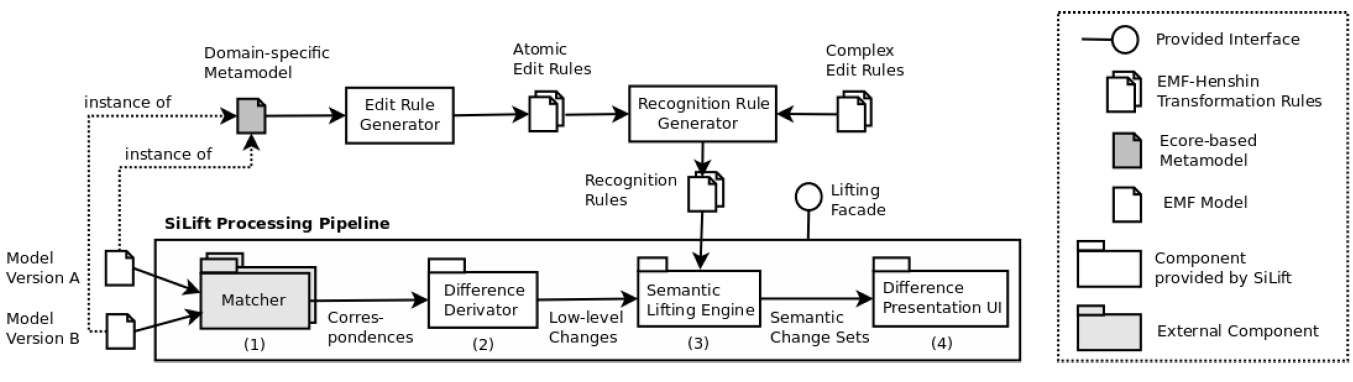
\includegraphics[width=\textwidth]{graphics/silift-processing_pipeline.png}
\caption{SiLift Processing Pipeline}
\label{silift-processing_pipeline}
\end{figure}

Die Vorgehensweise von SiLift lässt sich am besten mit einer vierstufigen \textit{Pipeline}, wie in Abbildung \ref{silift-processing_pipeline} dargestellt,  vergleichen.
Als Eingabe dienen immer zwei Versionen eines Modells:

\begin{enumerate}

\item \textbf{Matching}: 
Aufgabe eines \textit{Matcher} ist es, die korrespondierenden Elemente aus Modell A und Modell B, also die Elemente, die in beiden Modellen übereinstimmen, zu identifizieren.
Dabei ist das Ergebnis vor allem davon abhängig anhand welcher Kriterien der Matcher eine Übereinstimmung festlegt.
Hier wird unter anderem unterschieden zwischen \textit{ID-}, \textit{signatur-} und \textit{ähnlichkeitsbasierten} Verfahren.\\
In SiLift stehen standardmäßig folgende \textit{Matcher-Engines} zur Verfügung:

\begin{itemize}
	\item \texttt{EcoreID Matcher}: Ein \textit{ID-basierter} Matcher (nutzt Werte von Attributen, die im Metamodell als ID-Attribute deklariert sind).
	\item \texttt{EMF Compare}: 
	Unterstützt alle drei Verfahren. \texttt{EMF Compare} kann unter \texttt{Win\-dow} $\triangleright$ \texttt{Preferences}: \texttt{EMF Compare} konfiguriert werden. \footnote{Informationen zum \texttt{EMF Compare Project} finden Sie unter \url{http://www.eclipse.org/emf/compare}.}
	
	\item \texttt{NamedElement Matcher}: 
	Ein \textit{signaturbasierter} Matcher, welcher die ent\-sprech\-en\-den Korrespondenzen anhand der Werte der jeweiligen Namensattribute bestimmt.
	
	\item \texttt{URIFragment Matcher}: 
	Ein \textit{signaturbasierter} Matcher, welcher die ent\-sprech\-en\-den Korrespondenzen anhand der Werte der \textit{Uri} der Elemente bestimmt (z.B. \texttt{eType=}"'\texttt{ecore:EDataType http://www.eclipse.org/emf/2002""/Ecore""\#//EString}"').
	
	\item \texttt{UUID Matcher}: Ein \textit{ID-basierter Matcher} (basiert auf XMI-IDs der XMI-Repräsentationen der Modelle, falls vorhanden).
\end{itemize}

Diese Liste ist keineswegs abgeschlossen und kann durch zusätzliche Matching-Engines, wie z.B. \textit{SiDiff} oder auch eigener Matcher ergänzt werden (siehe Abschnitt \ref{sec:own_matching_engine}). \\

\item \textbf{Difference derivation}: 
Ausgehend von den gefunden Korrespondenzen berechnet der \textit{Difference Derivator} eine technische Differenz (\textit{low-level difference}) der Mo\-del\-le.
Alle Objekte und Referenzen, für die keine Korrespondenz existiert müssen demnach entweder in Modell B hinzugefügt, oder aus Modell A entfernt worden sein.

\item \textbf{Semantic Lifting}:\label{page:semantic_change_sets}
Die zuvor berechnete technische Differenz enthält alle Än\-der\-ung\-en  auf Basis des Metamodells.
Diese sollen nun semantisch geliftet werden.
Bei einer \textit{semantisch gelifteten Differenz} handelt es um eine halbgeordnete Menge von auf einem vorhandenen Modell (dem Basismodell) ausgeführten \textit{Editieroperationen}.
Durch das liften der technischen Differenz werden die einzelnen Änderungen mit Hilfe von \textit{Erkennungsregeln} (engl. \textit{recognition rules}) in sogenannte \textit{Semantic Change Sets} gruppiert. Diese repräsentieren wiederum jeweils eine vom Benutzer ausgeführte Editieroperation.
Das Verhalten einer Editieroperation wird durch die zugehörige \textit{Editierregel} definiert, aus denen sich mit Hilfe des \textit{Recognition Rules Generators} die Erkennungsregeln ableiten lassen. 
Was wiederum eine gültige bzw. sinnvolle Editierregel ist hängt zum einem vom Metamodell, zum anderen von den Benutzerpräferenzen ab. 
Daher lassen sich die Editierregeln und somit auch die Erkennungsregeln grob zweier sogenannter Regelbasen (engl. \textit{Rule Bases}) zuordnen:

\begin{itemize}
\item \textbf{\texttt{Atomic Rule Base}}: 
Atomare Regeln umfassen das Erzeugen (engl. \textit{create}), Löschen (engl. \textit{delete}), Verschieben von Elementen (engl. \textit{move}) sowie das Ändern von Attributwertenv(engl. \textit{change}).
Sie lassen sich nicht in kleinere Teile zerlegen, ohne dass deren Anwendung zu einem inkonsistenten Modell führen würde.\\
Atomaren Regeln können mit Hilfe eines \textit{Editrulegenerators}\footnote{Weitere Information zum Editrulegenerator finden Sie unter \url{http://pi.informatik.uni-siegen.de/Projekte/SERGe.php}.} direkt aus dem Metamodell abgeleitet werden. 
Problematisch wird es, wenn weitere Restriktionen (engl. \textit{Constraints}), wie sie bspw. die UML in Form von \textit{OCL-Ausdrücken} benutzt, die Konsistenzkriterien eines Modells bzw. dessen Elemente weiter eingrenzen. 
I.d.R. werden diese nicht bei der Implementierung eines Metamodells berücksichtigt.
Hier bleibt nur die Möglichkeit die Regeln manuell zu editieren bzw. anzupassen.

\item \textbf{\texttt{Complex Rule Base}}: 
Die komplexen Editierregeln setzen sich i.d.R. aus den atomaren und anderen komplexen Regeln zusammen und beschreiben umfangreichere Editieroperationen, welche vor allem beim \textit{Refactoring} auftreten. 
Da solche Refactorings sehr benutzerspezifisch sind müssen komplexe Regeln generell von Hand erstellt werden.
\end{itemize}

\item \textbf{Difference Presentation UI}:
SiLift stellt zwei Benutzerschnittstellen (engl. \textit{User Interfaces}) zur Verfügung, um die semantisch gelifteten Differenzen anzuzeigen: 
einen Baum-basierten  und einen grafischen Editor, in dem die Differenzen \textit{gehighlightet} werden.\footnote{Beispielansichten finden Sie im \textbf{SiLift - Benutzerhandbuch für Endanwender}}
\end{enumerate}

%*************************************************************************
\section{Integration eigener Matching-Engines} \label{sec:own_matching_engine}
%*************************************************************************

Wie bereits erwähnt lassen sich auch eigene Matching-Engines in die SiLift-Processing-Pipeline integrieren.\\
Erstellen Sie dazu über \texttt{File} $\triangleright$ \texttt{New} $\triangleright$ \texttt{Other...}: \texttt{Plug-in Development} $\triangleright$ \texttt{Plug-in Project} eines neues Plugin und öffnen Sie die \texttt{MANIFEST.MF}.
Wechseln Sie auf den Reiter \texttt{Dependencies} und fügen Sie die in Abbildung \ref{silift-plugin_matcher_manifest_dependencies} markierten Abhängigkeiten hinzu.

\begin{figure}[H]
\centering
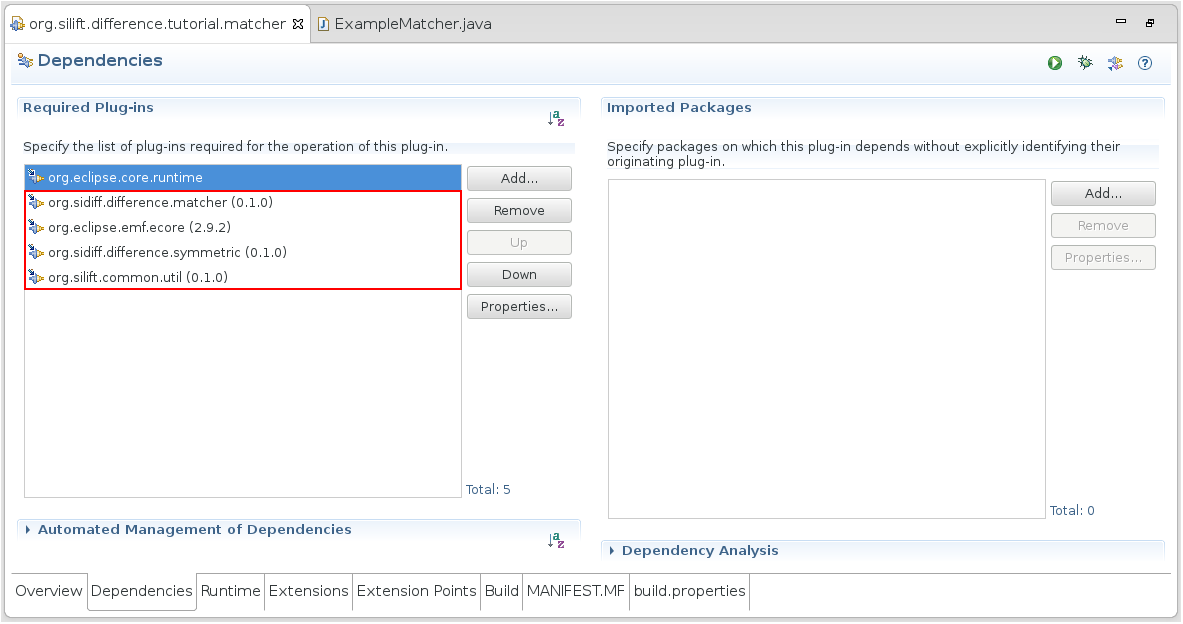
\includegraphics[width=0.8\textwidth]{graphics/silift-plugin_matcher_manifest_dependencies}
\caption{\texttt{MANIFEST.MF} $\triangleright$ \texttt{Dependencies}}
\label{silift-plugin_matcher_manifest_dependencies}
\end{figure}

Als nächstes wird eine Klasse benötigt die die Schnittstelle \texttt{IMatcher} implementiert (vgl. Abb. \ref{silift-plugin_matcher_imatcher}).
Neben den zu implementierenden Methoden ist es Ihnen frei gestellt, ob sie Ihren Matcher in dieser Klasse implementieren oder diese nur als Adapter für einen ausgelagerten Matcher nutzen.

\begin{figure}[H]
\centering
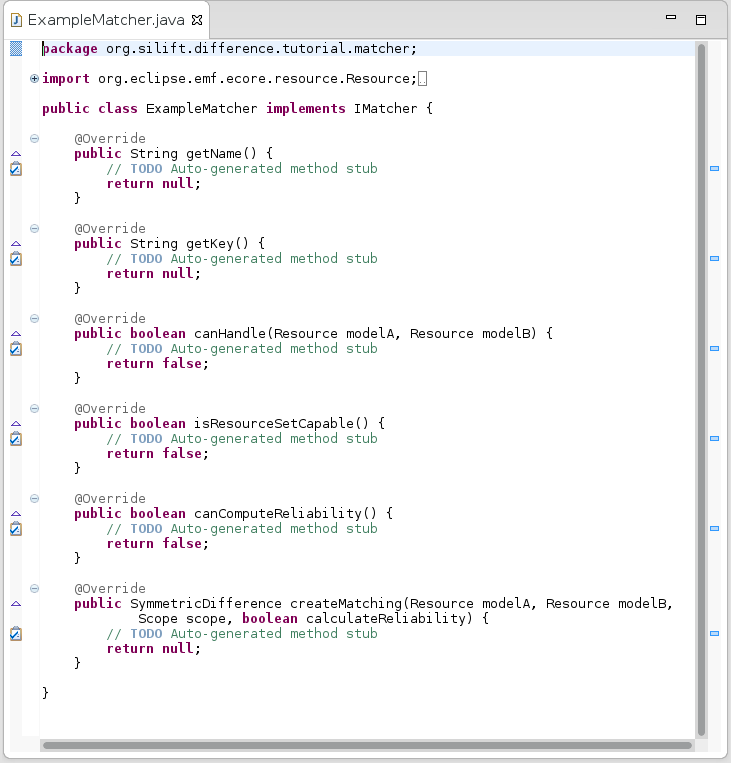
\includegraphics[width=0.6\textwidth]{graphics/silift-plugin_matcher_imatcher.png}
\caption{Klasse \texttt{ExampleMatcher} implementiert \texttt{IMatcher}}
\label{silift-plugin_matcher_imatcher}
\end{figure}

Anstatt die Schnittstelle \texttt{IMatcher} von Grund auf zu implementieren, kann auch die ``Convenience''-Klasse \texttt{BaseMatcher} erweitert werden (vgl. Abb. \ref{silift-plugin_matcher_basematcher}).
Diese stellt bereits Methoden zum Iterieren über die Modellelemente bereit.
Zusätzlich muss noch die Methode \texttt{isCorresponding} implementiert werden.

\begin{figure}[H]
\centering
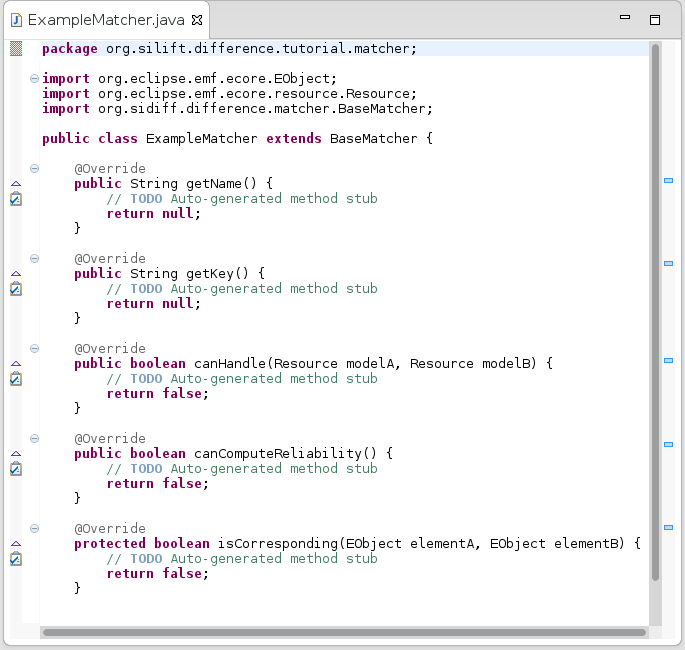
\includegraphics[width=0.6\textwidth]{graphics/silift-plugin_matcher_basematcher.png}
\caption{Klasse \texttt{ExampleMatcher} erweitert \texttt{BaseMatcher}}
\label{silift-plugin_matcher_basematcher}
\end{figure}

Danach muss das Plugin noch als Extension für \texttt{SiLift} definiert werden.
Gehen Sie dazu wieder in die \texttt{MANIFEST.MF} und wechseln Sie auf den Reiter \texttt{Extensions} (vgl. Abb. \ref{silift-plugin_manifest_extensions}).

\begin{figure}[H]
\centering
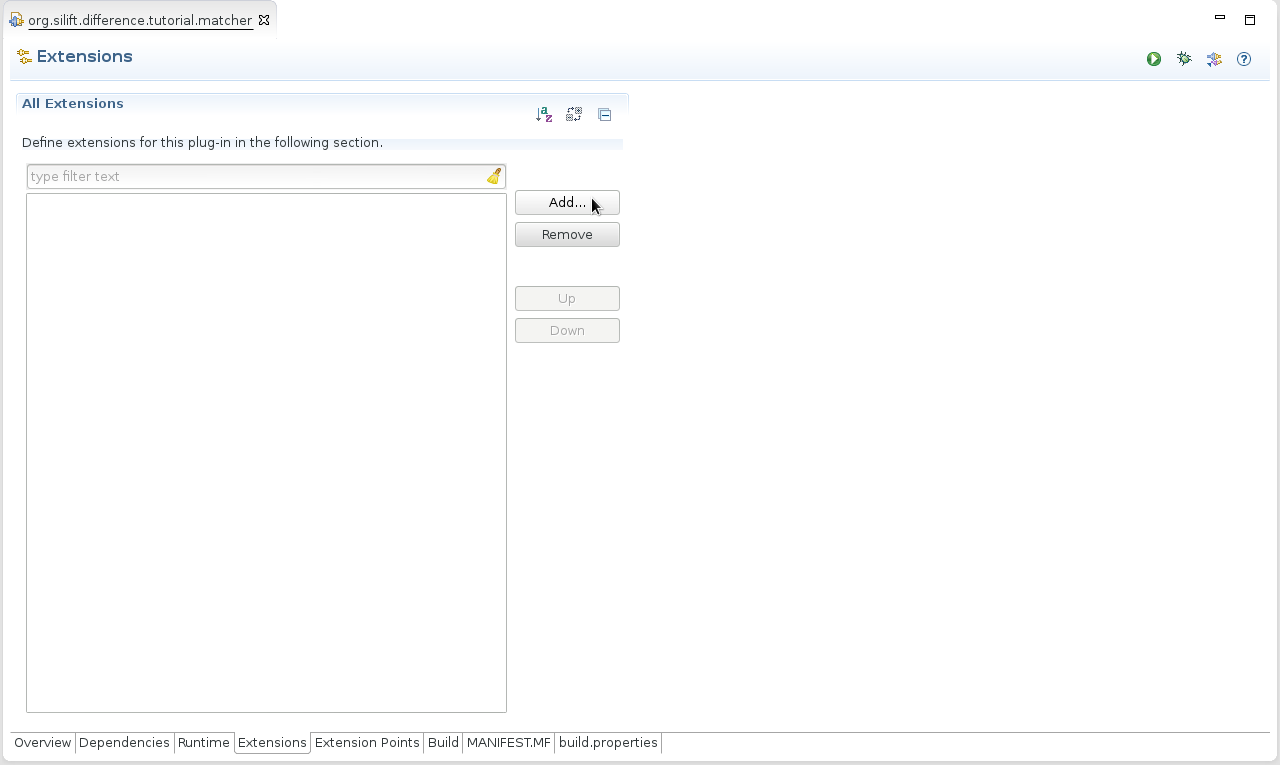
\includegraphics[width=0.8\textwidth]{graphics/silift-plugin_manifest_extensions.png}
\caption{\texttt{MANIFEST.MF} $\triangleright$ \texttt{Extensions}}
\label{silift-plugin_manifest_extensions}
\end{figure}

Klicken Sie auf auf \texttt{Add...} und selektieren Sie den \textit{Extension Point} \texttt{org.""sidiff.""difference.""matcher.""matcher\_""extension} (vgl. Abb. \ref{silift-plugin_manifest_add_extension_point}).

\begin{figure}[H]
\centering
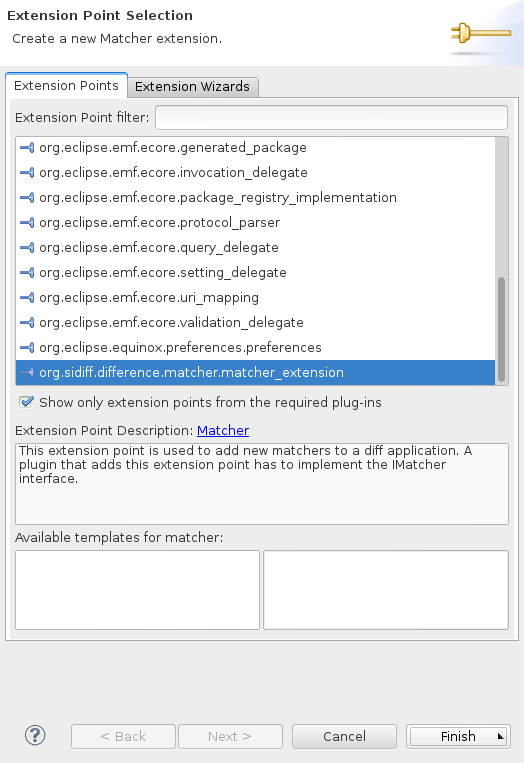
\includegraphics[width=0.6\textwidth]{graphics/silift-plugin_manifest_add_extension_point.png}
\caption{\texttt{MANIFEST.MF} $\triangleright$ \texttt{Extensions}: Extension Point Selection}
\label{silift-plugin_manifest_add_extension_point}
\end{figure}

Wechseln Sie in den Reiter \texttt{plugin.xml} und fügen dem eben erstellen Extension Point die entsprechende URI der Erweiterung bei (vgl. Abb. \ref{silift-plugin_manifest_plugin}).

\begin{figure}[H]
\centering
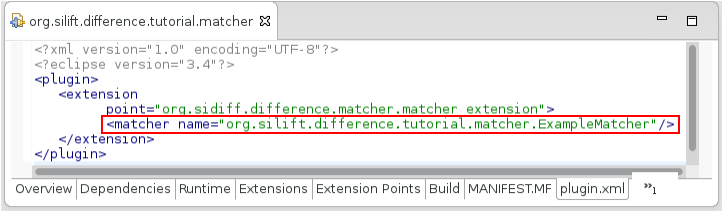
\includegraphics[width=0.6\textwidth]{graphics/silift-plugin_manifest_plugin.png}
\caption{\texttt{MANIFEST.MF} $\triangleright$ \texttt{plugin.xml}}
\label{silift-plugin_manifest_plugin}
\end{figure}

Als letztes muss das Plugin noch \textit{deployed} werden.
Öffnen Sie mit der rechten Maustaste auf Ihrem Plugin-Projekt im Package Exploerer das Kontextmenü und klicken Sie auf \texttt{Export...} (vgl. Abb. \ref{silift-plugin_contextmenu_export}).
%Als letztes muss das Plugin noch in den \texttt{dropins}-Ordner von Eclipse exportiert werden (vgl. Abschnitt \ref{sec:deploying_recognitionrules}).

\begin{figure}[H]
\centering
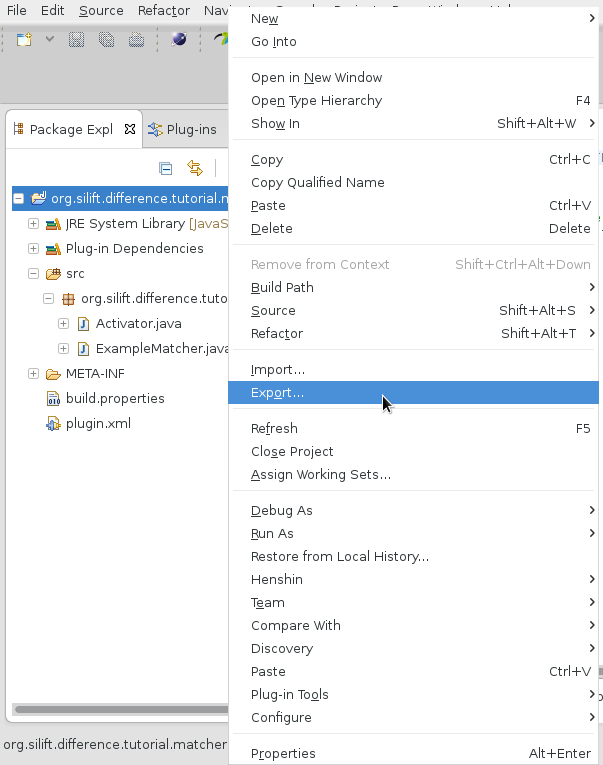
\includegraphics[width=0.6\textwidth]{graphics/silift-plugin_contextmenu_export.png}
\caption{\texttt{Export Plugin}}
\label{silift-plugin_contextmenu_export}
\end{figure}

Selektieren Sie \texttt{Plug-in Development} $\triangleright$ \texttt{Deployable plug-ins and fragements} und klicken Sie \texttt{Next} (vgl. Abb. \ref{silift-plugin_wizard_deploy01}).

\begin{figure}[H]
\centering
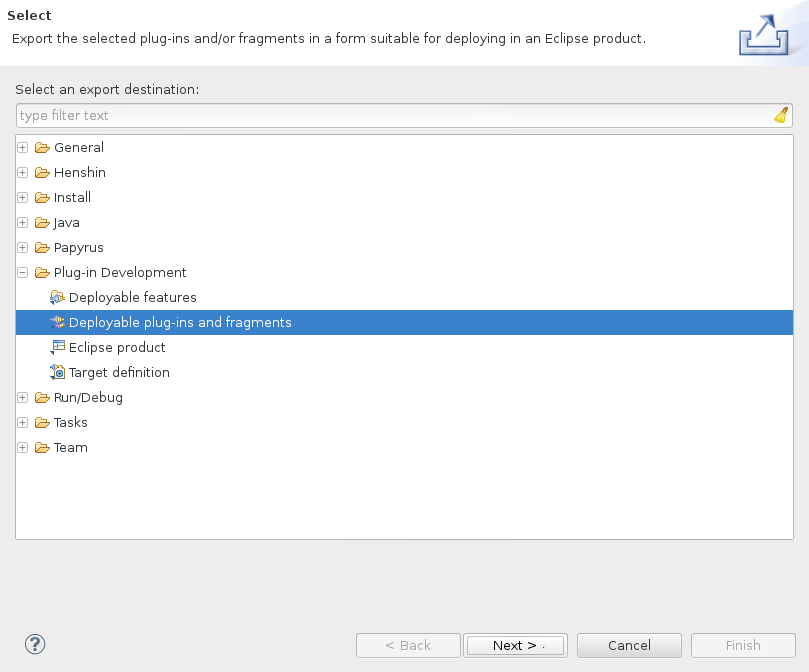
\includegraphics[width=0.6\textwidth]{graphics/silift-plugin_wizard_deploy01.png}
\caption{\texttt{Export Wizard}: Page 1}
\label{silift-plugin_wizard_deploy01}
\end{figure}

Wählen Sie als nächstes \texttt{install into host.Repository} aus und geben Sie den Pfad zum Plugin-Ordner Ihrer Eclipse-Installation an (vgl. Abb. \ref{silift-plugin_wizard_deploy02}).
Klicken Sie auf \texttt{Finish} und starten Sie nach erfolgreicher Installation Ihr Eclipse neu.

\begin{figure}[H]
\centering
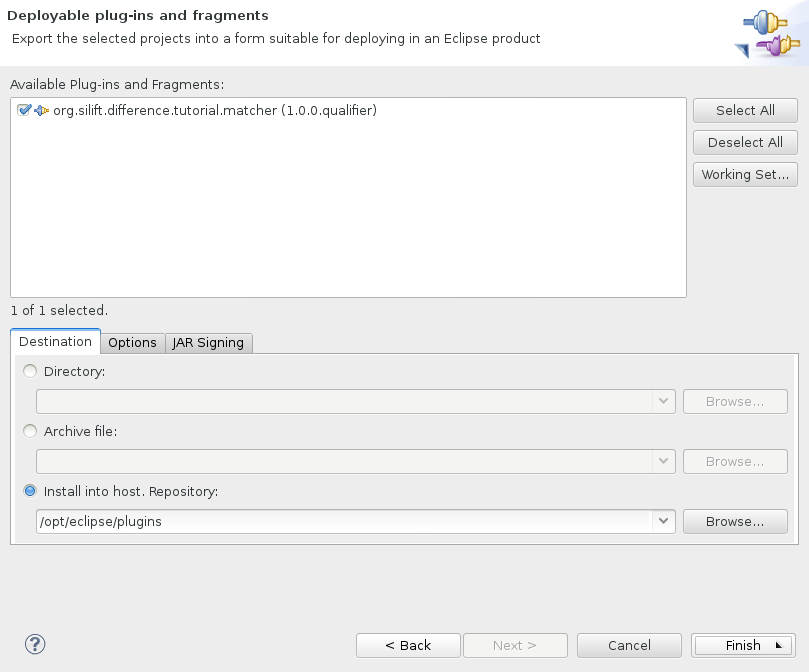
\includegraphics[width=0.6\textwidth]{graphics/silift-plugin_wizard_deploy02.png}
\caption{\texttt{Export Wizard}: Page 2}
\label{silift-plugin_wizard_deploy02}
\end{figure}

Ihr Matcher kann nun in Verbindung mit SiLift genutzt werden.

%*************************************************************************
\section{Erstellen eines Technical Difference Builders}\label{sec:TechnicalDifferenceBuilder}
%*************************************************************************

Ein Matcher kann i.d.R. für mehrere Modelle unterschiedlichen Typs benutzt werden. Dahingegen muss für jeden Modelltyp (Metamodell) ein separater \textit{Technical Difference Builder} erzeugt werden.\\
Erstellen Sie dazu über \texttt{File} $\triangleright$ \texttt{New} $\triangleright$ \texttt{Other...}: \texttt{Plug-in Development} $\triangleright$ \texttt{Plug-in Project} eines neues Plugin und öffnen Sie die \texttt{MANIFEST.MF}.
Wechseln Sie auf den Reiter \texttt{Dependencies} und fügen Sie die in Abbildung \ref{silift-plugin_techbuilder_manifest_dependencies} gelisteten Abhängigkeiten hinzu.

\begin{figure}[H]
\centering
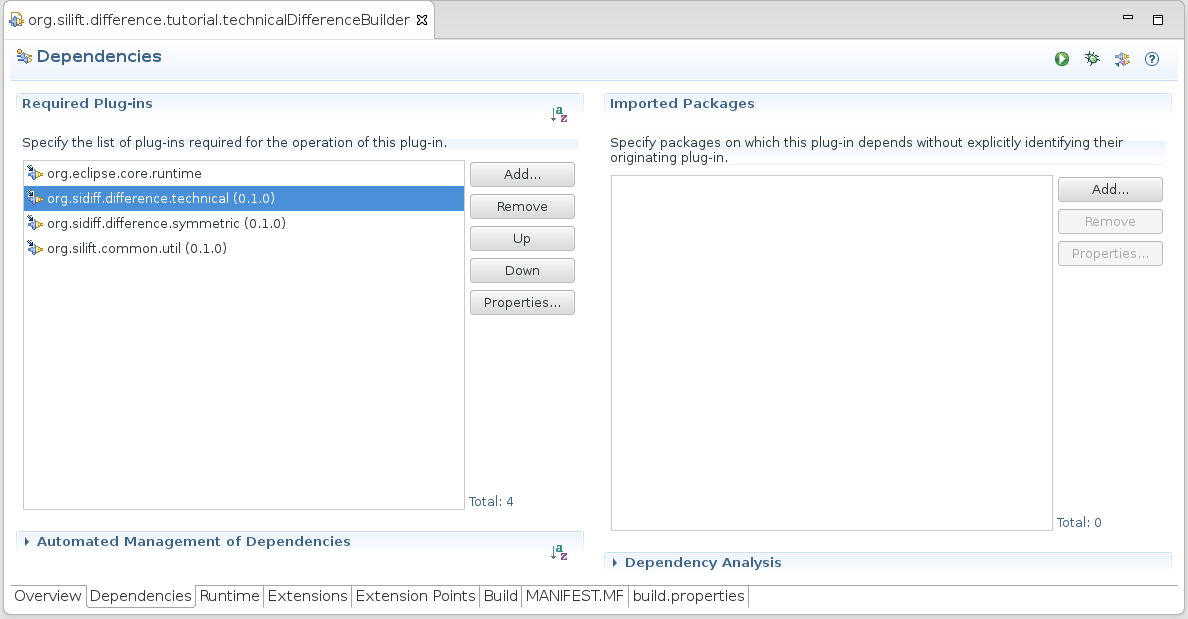
\includegraphics[width=0.8\textwidth]{graphics/silift-plugin_techbuilder_manifest_dependencies.png}
\caption{\texttt{\texttt{MANIFEST.MF} $\triangleright$ \texttt{Dependencies}}}
\label{silift-plugin_techbuilder_manifest_dependencies}
\end{figure}

Als nächstes wird eine Klasse benötigt die die Schnittstelle \texttt{ITechnicalDifferenceBuilder} implementiert (vgl. Abb. \ref{silift-plugin_techbuilder_itechbuilder}).

\begin{figure}[H]
\centering
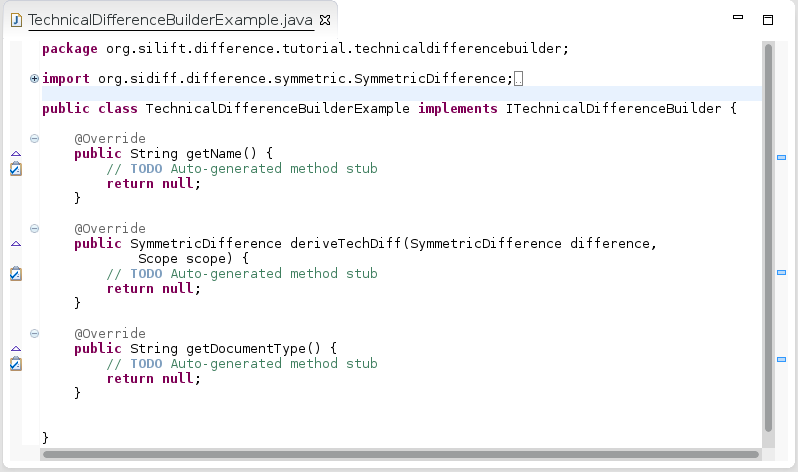
\includegraphics[width=0.6\textwidth]{graphics/silift-plugin_techbuilder_itechbuilder.png}
\caption{Klasse \texttt{TechnicalDifferenceBuilderExample} implementiert \texttt{ITechnicalDifferenceBuilder}}
\label{silift-plugin_techbuilder_itechbuilder}
\end{figure}

Anstatt die Schnittstelle \texttt{ITechnicalDifferenceBuilder} von Grund auf zu implementieren, kann auch die ``Convenience''-Klasse \texttt{Technical\-Difference\-Builder} erweitert werden.\\
Diese implementiert bereits die Methode \texttt{deriveTechDiff}. Durch die manuelle Implementierung der Methoden \texttt{getUnconsideredNodeTypes}, \texttt{getUnconsideredEdgeTypes} und \texttt{getUnconsideredAttributeTypes} können zudem Modellelemente gefiltert und somit von der Differenzbildung ausgeschlossen werden (vgl. Abb. \ref{silift-plugin_techbuilder_techbuilder}).


\begin{figure}[H]
\centering
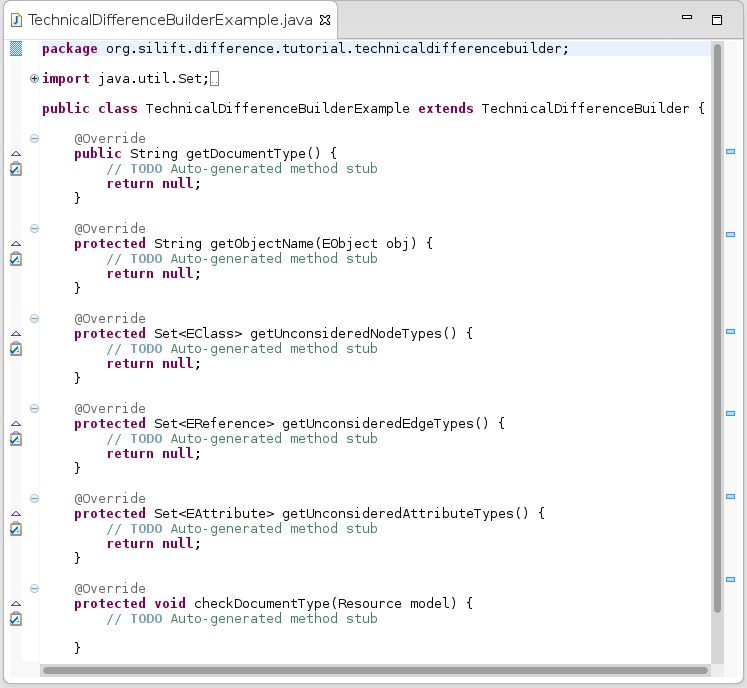
\includegraphics[width=0.6\textwidth]{graphics/silift-plugin_techbuilder_techbuilder.png}
\caption{\texttt{Klasse \texttt{TechnicalDifferenceBuilderExample} erweitert \texttt{TechnicalDifferenceBuilder}}}
\label{silift-plugin_techbuilder_techbuilder}
\end{figure}

Danach muss das Plugin analog zu Abschnitt \ref{sec:own_matching_engine} noch als Extension für \texttt{SiLift} definiert werden.
Gehen Sie dazu wieder in die \texttt{MANIFEST.MF} und wechseln Sie auf den Rei\-ter \texttt{Extensions}. Klicken Sie auf auf \texttt{Add...} und selektieren Sie den \textit{Extension Point} \texttt{org.sidiff.difference.technical.technical\_difference\_builder\_extension} .\\
Klicken sie danach mit der rechten Maustaste auf die Extension und wählen sie \texttt{New} $\triangleright$ \texttt{technical} (vgl. Abb. \ref{silift-plugin_techbuilder_manifest_extension_point}).

\begin{figure}[H]
\centering
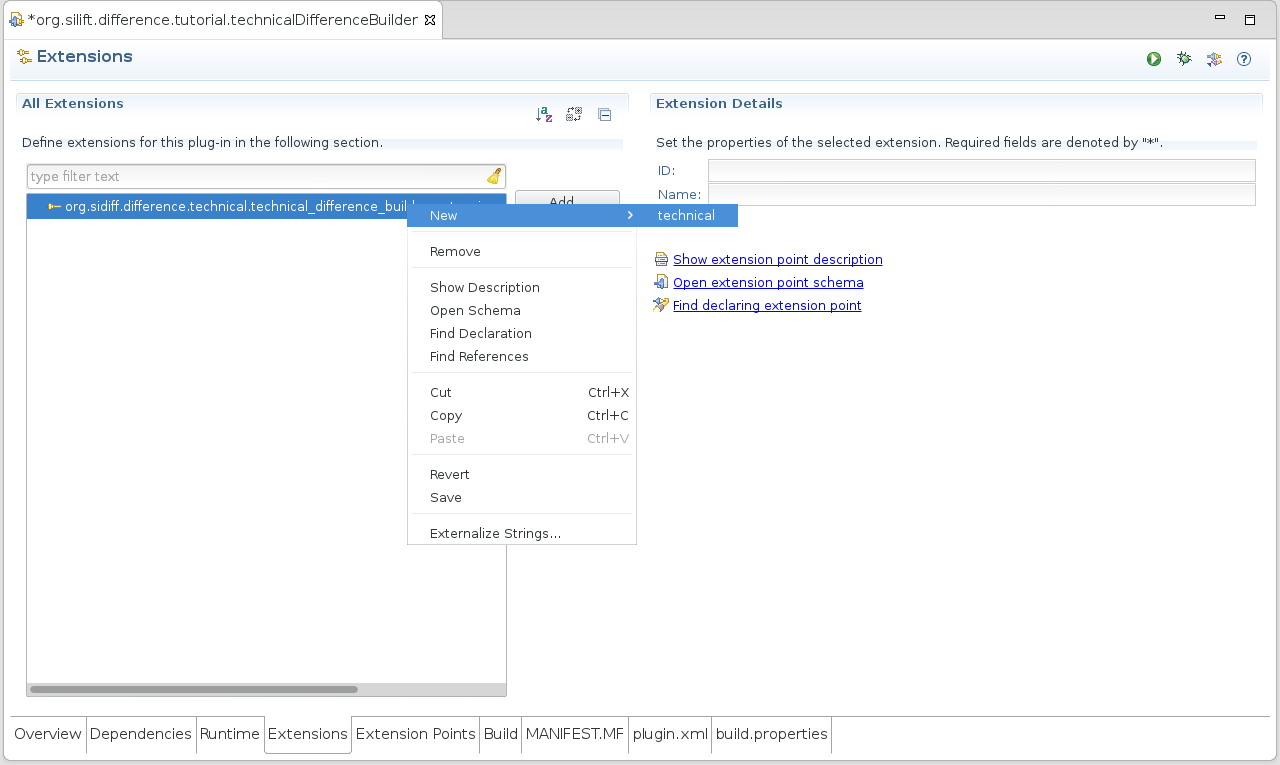
\includegraphics[width=0.8\textwidth]{graphics/silift-plugin_techbuilder_manifest_extension_point.png}
\caption{\texttt{Klasse \texttt{MANIFEST.MF} $\triangleright$  \texttt{Extensions}}}
\label{silift-plugin_techbuilder_manifest_extension_point}
\end{figure}

Als letztes müssen Sie noch unter \texttt{Extension Element Details} $\triangleright$ \texttt{difference\_builder} Ihre zuvor erstellte Klasse eingeben (vgl. Abb. \ref{silift-plugin_techbuilder_manifest_dependencies}).

\begin{figure}[H]
\centering
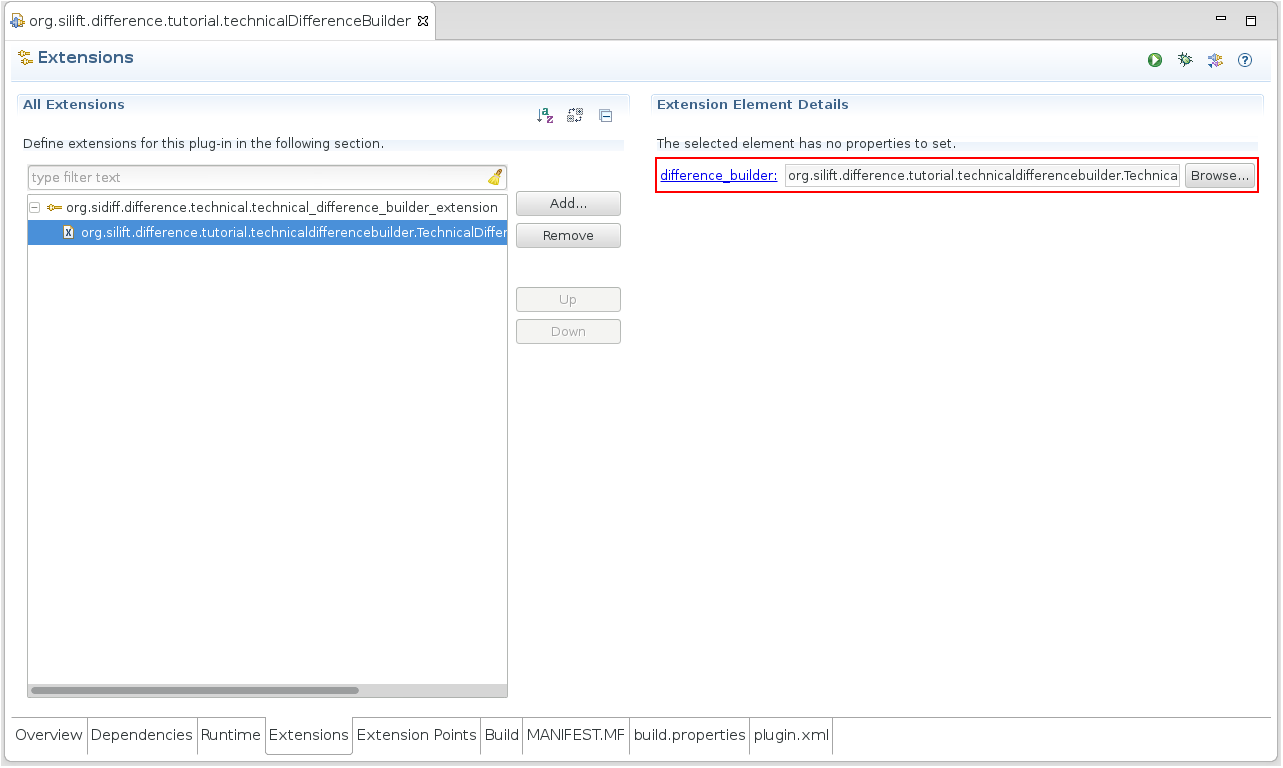
\includegraphics[width=0.8\textwidth]{graphics/silift-plugin_techbuilder_manifest_extension.png}
\caption{\texttt{Klasse \texttt{MANIFEST.MF} $\triangleright$  \texttt{Extensions}: \texttt{difference builder}}}
\label{silift-plugin_techbuilder_manifest_extension}
\end{figure}

Damit SiLift Ihren Difference Builder findet muss dieser noch analog zu Abschnitt \ref{sec:own_matching_engine} deployed werden.

%*************************************************************************
\section{Erstellen von Editierregeln}
%*************************************************************************

%Mit \textit{SiLift} können Differenzen von \textit{EMF-basierten} Modellen, d.h. Modelle die auf dem \textit{Ecore-Metamodell} basieren, semantisch geliftet werden.
%Für \textit{domainspezifische} Modellierungssprachen bedeutet das, dass deren Metamodell zuerst in ein entsprechendes \textit{Ecore-Modell} übertragen werden muss, bevor Editierregeln implementiert und Erkennungsregeln abgeleitet werden können.\\

\subsection{Metamodell}\label{subsec:metamodel}
Abbildung \ref{statemachine_metamodel} stellt ein Metamodell für \textit{Zustandsautomaten} (engl. \textit{statemachines}) ähnlich dem der UML dar.

\begin{figure}[H]
\centering
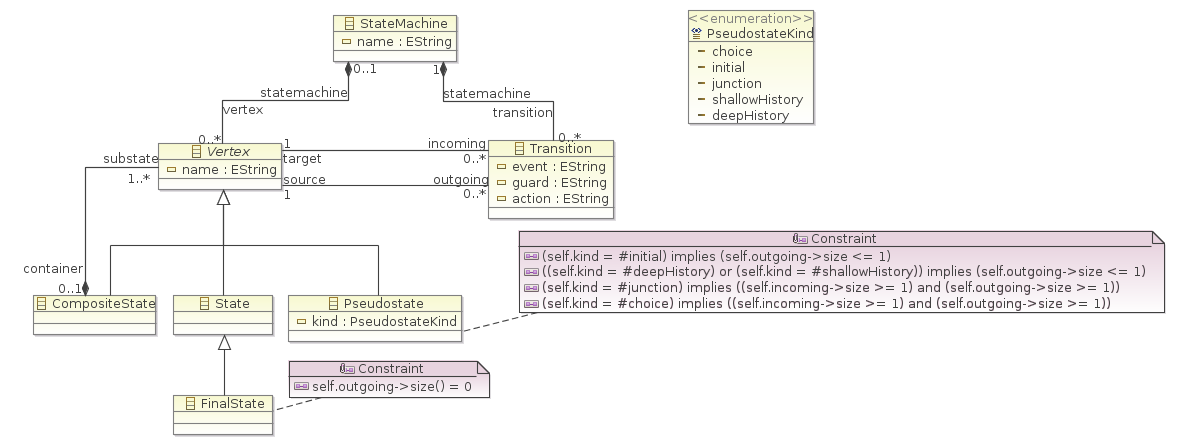
\includegraphics[width=\textwidth]{graphics/statemachine.png}
\caption{Zustandsautomat Metamodell}
\label{statemachine_metamodel}
\end{figure}

Ein \textit{Zustandsautomat} (\texttt{StateMachine}) besteht aus einer endlichen Anzahl von \textit{Zuständen} (\texttt{Vertex}) und \textit{Transitionen} (\texttt{Transition}).
Bei den Zuständen wird zwischen \textit{normalen Zuständen} (\texttt{State}), \textit{Pseudozuständen} (\texttt{Pseudostate}), \textit{Endzuständen} (\texttt{FinalState}) und \textit{zusammengesetzten Zuständen} (\texttt{CompositeState}) unterschieden.
Eine \textit{Transition} verbindet immer zwei Zustände und  kann ein \textit{Ereignis} (\texttt{Event}),  eine \textit{Bedingung} (\texttt{Guard}) und einer \textit{Aktion} (\texttt{Action}) besitzen.\\
Neben den Kardinalitäten der Referenzen sind weitere Konsistenzkriterien durch \textit{OCL-Ausdrücke} definiert. 
So darf z.B. eine Startzustand (\texttt{PseudostateKind: initial}) keine eingehende und maximal eine ausgehende Transition besitzen.\\
Im Folgendem lernen Sie ausgehend von dem vorgestellten Metamodell Editierregeln mit Hilfe von \textit{Henshin-Regeln} zu erstellen.\\



\textbf{Hinweis}: SiLift unterstützt momentan nur \textit{statisches EMF}, d.h. dass das Metamodell als \textit{Eclipse-Plugin} "'\textit{deployed}"' sein muss.


\subsection{Exkurs in EMF-Henshin}

Bei \textit{Henshin} handelt es sich um eine Transformationsprache bzw. ein Graphersetzungssystem für \textit{EMF Modelle}. 
Modelle werden als \textit{Graphen} interpretiert (man spricht hier auch von dem Arbeitsgraphen, der das Modell repräsentiert) und nach \textit{Teilgraphen} durchsucht, die vorher in einer sogenannten \textit{Transformationsregeln} definiert wurden.
Man spricht bei diesem Teilgraphen von der \textit{Left-Hand Side} (kurz \textit{LHS}) der Trans\-for\-ma\-tions\-re\-gel. 
Wird ein solcher Teilgraph gefunden wird er durch die sogenannte \textit{Right-Hand Side} (kurz \textit{RHS}) der Transformationsregel ersetzt. 
Dabei werden die Knoten und Kanten, die in der linken und nicht in der rechten Seite vorkommen gelöscht und die, die in der rechten Seite und nicht in der linken vorkommen werden erzeugt.
Knoten, die in beiden Seiten vorkommen bleiben unverändert.
Man spricht bei diesen Knoten auch vom Kontext der Transformationsregel.
Dieser Kontext kann durch sogenannte \textit{Negative Application Conditions} (kurz \textit{NACs}) weiter eingeschränkt werden.\footnote{Einführende Beispiele finden Sie unter \url{http://www.eclipse.org/henshin/examples.php}.}\\
Mehrere Regeln lassen sich in einem \textit{Modul} (engl. \textit{module}) zusammenfassen, wobei die Reihenfolge der Ausführung der Regeln durch sogenannte \textit{Units} bestimmt wird: \texttt{Independent Unit}, \texttt{Sequential Unit}, \texttt{Conditional Unit}, \texttt{Priority Unit}, \texttt{Iterated Unit} und \texttt{Loop Unit}.\\

\textbf{Hinweis}: Momentan verlangt SiLift für jede Editieroperation immer ein Transformationssystem mit genau einer \textit{mainUnit} (\texttt{Independent}, \texttt{Priority} oder \texttt{Sequential}) und einer darin enthaltenen Regel. Eine Ausnahme bilden geschachtelte Regeln, in der eine \textit{Kernel-Regel} und eine beliebige Menge von \textit{Multi-Regeln} definiert werden.


Henshin stellt zum Entwickeln von Transformationsystemen zwei Editoren zur Verfügung:

\begin{enumerate}

\item \textbf{Henshin Transformation Model Editor}: 
Ein baumbasierter Editor mit ent\-sprech\-en\-der linken und rechten Seite der Transformationsregeln (vgl. Abb.\ref{silift-editrule_createStateInStateMachine}: links).

\item \textbf{Henshin Diagram Editor}: 
Ein graphenbasierter Editor mit den \textit{"'Stereotypen"'} \texttt{create}, \texttt{delete}, \texttt{preserve}, \texttt{require} und \texttt{forbid} zum markieren entsprechender Operationen (vgl. Abb. \ref{silift-editrule_createStateInStateMachine}: rechts).
Knoten und Kanten die mit \texttt{delete} markiert sind, kommen nur in der \textit{LHS} vor, wohingegen Knoten und Kanten, die mit \texttt{create} markiert sind nur in der \textit{RHS} vorkommen.
Knoten, die auf beiden Seiten vorkommen werden als \texttt{preserve} markiert.
Mit \texttt{require} und \texttt{forbid} lassen sich Teilgraphen erzeugen, die in einem Kontext auftreten müssen bzw. nicht auftreten dürfen.
\end{enumerate}


\subsection{Atomare Editierregeln}

Wie bereits erwähnt umfassen die atomaren Regeln das Erzeugen, Löschen, Verschieben von Elementen und das Ändern von Attributwerten.
Um eine Editierregel zu erstellen legen Sie ein neues Projekt an und wählen Sie \texttt{File} $\triangleright$ \texttt{New} $\triangleright$ \texttt{Other...} und hier \texttt{Henshin Model} aus. 
Klicken Sie auf \texttt{Next} (vgl. Abb. \ref{silift-create_henshin_model_page01}).\\
%Im nächsten Dialog wird nach einem Dateinamen gefragt. 


\begin{figure}[H]
\centering
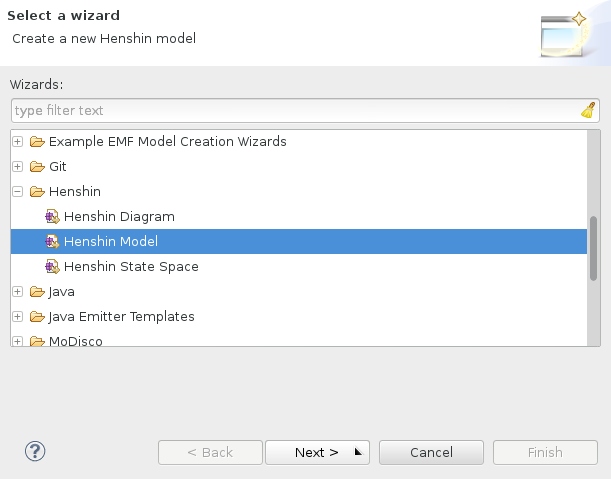
\includegraphics[width=0.6\textwidth]{graphics/silift-create_henshin_model_page01.png}
\caption{Erstellen eines neuen Transformationsmodells: Page 1}
\label{silift-create_henshin_model_page01}
\end{figure}

Die Datei kann einen beliebigen Namen bekommen, jedoch muss sie auf \texttt{\_execute.henshin} enden.
Da der Name der Regel eindeutig sein muss ist es zu empfehlen die Datei nach ihrer späteren Regel zu benennen. Somit behalten Sie den Überblick.
Die folgende Regel soll einen Zustand in einen vorhanden Zustandsautomaten einfügen. Hier würde sich bspw. der Name \texttt{Create\_StateInStateMachine\_execute.henshin} anbieten (vgl. Abb.\ref{silift-create_henshin_model_page02}).
Wählen sie den Zielordner und geben Sie den Dateinamen ein.
Klicken Sie auf \texttt{Next}.

\begin{figure}[H]
\centering
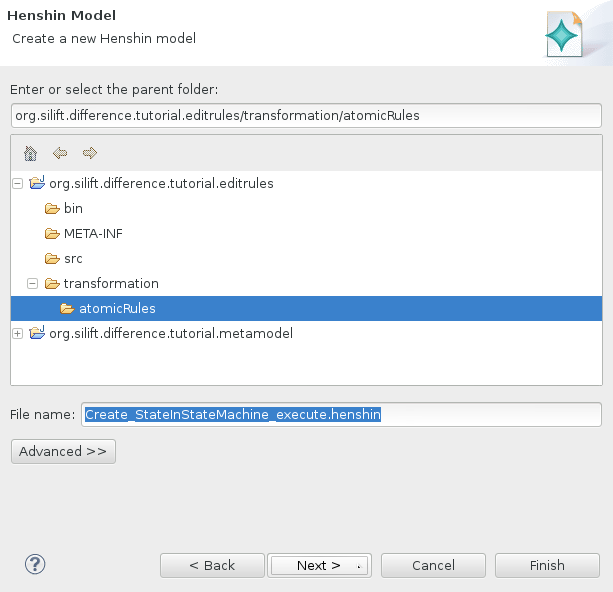
\includegraphics[width=0.6\textwidth]{graphics/silift-create_henshin_model_page02.png}
\caption{Erstellen eines neuen Transformationsmodells: Page 2}
\label{silift-create_henshin_model_page02}
\end{figure}

Als letztes müssen Sie noch Ihr Metamodel aus der Registry (\texttt{Add From Registry}) laden (vgl. Abb. \ref{silift-create_henshin_model_page03}).

\begin{figure}[H]
\centering
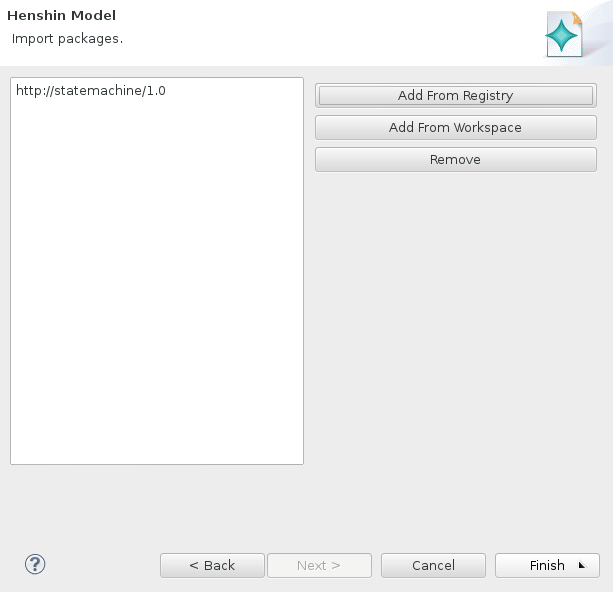
\includegraphics[width=0.6\textwidth]{graphics/silift-create_henshin_model_page03.png}
\caption{Erstellen eines neuen Transformationsmodells: Page 3}
\label{silift-create_henshin_model_page03}
\end{figure}

Um neben dem baumbasierten auch den graphenbasierten Editor nutzen zu können muss zusätzlich noch ein \textit{Henshin-Diagramm} erzeugt werden.
Klicken Sie hierzu mit der rechten Maustaste auf die \texttt{CREATE\_StateInStateMachine\_execute.henshin}, wählen Sie \texttt{Henshin} $\triangleright$ \texttt{Initialize Diagram File} aus und folgen Sie dem Assistenten (vgl. Abb. \ref{silift-initialize_henshin_diagram}).

\begin{figure}[H]
\centering
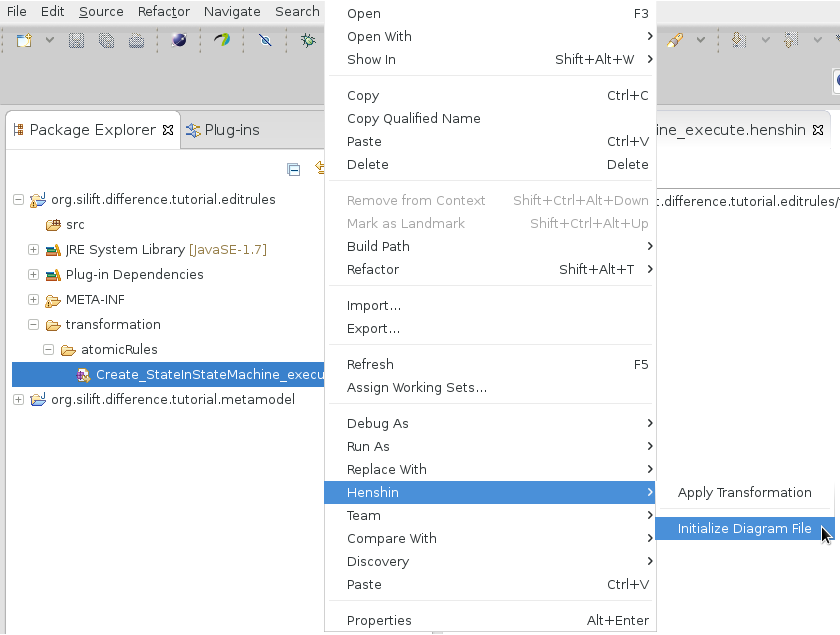
\includegraphics[width=0.5\textwidth]{graphics/silift-initialize_henshin_diagram.png}
\caption{Erstellen eines Henshin Diagramms}
\label{silift-initialize_henshin_diagram}
\end{figure}

%Als nächstes müssen Sie das Metamodell importieren.
%Klicken Sie dazu mit der rechten Maustaste in den Editor und wählen Sie  \texttt{import Package...} $\triangleright$  \texttt{From Registry} aus (vgl. Abb. \ref{henshin_import_metamodel_and_package_selection}).
%\vspace*{10mm}

%\begin{small}
%\textbf{WICHTIG}: Importieren Sie die \textit{Runtime Version} des Metamodells, damit später die Typen in der Editierregel über die \textit{NS-URI} lokalisiert werden.
%\end{small}
%\vspace*{5mm}

%\begin{figure}[H]
%\centering
%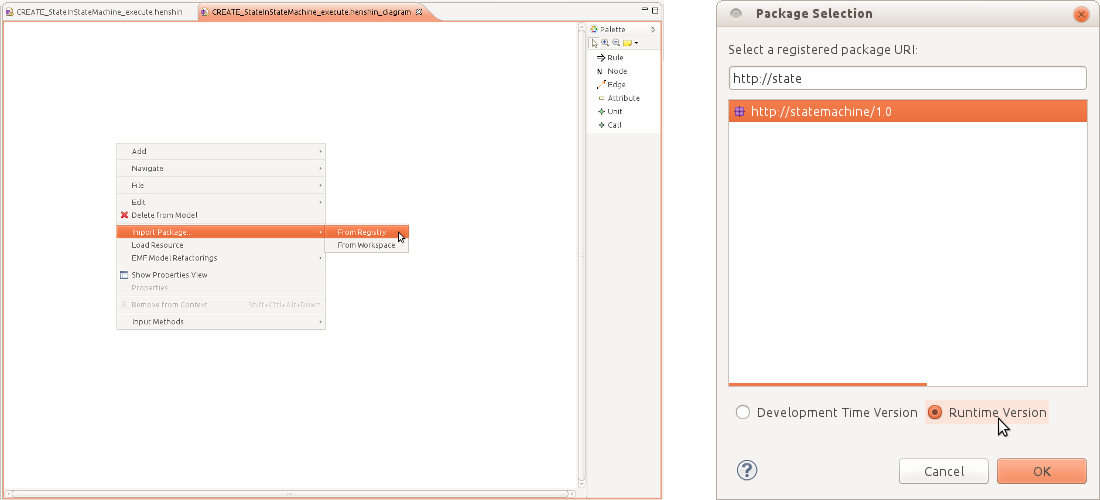
\includegraphics[width=0.8\textwidth]{graphics/henshin-import_metamodel_and_package_selection.png}
%\caption{Importieren des Metamodells}
%\label{henshin_import_metamodel_and_package_selection}
%\end{figure}

\subsubsection*{Create-Regeln}

Erstellen Sie eine Regel, indem sie aus der Palette das \textit{Rule-Werkzeug} auswählen und danach auf die Arbeitsfläche klicken. Geben Sie der Regel den Namen \texttt{create""State""In""State""Machine}.
Einer Regel können ähnlich einer Funktion oder Methode Parameter übergeben werden (vgl. Abb. \ref{silift-editrule_createStateInStateMachine}).
Dabei lässt sich zwischen \textit{Object-} und \textit{Value-Parametern} unterscheiden:

\begin{itemize}

\item \textbf{Object-Parameter}: 
Durch Objekt-Parameter können Objekte an die Regel über\-ge\-ben werden, um diese gezielt aus dem Arbeitsgraphen zu löschen, in dem Arbeitsgraphen zu erzeugen oder zu verändern.
Des Weiteren können dadurch Kontextobjekte eindeutig bestimmt werden. 
Sofern der Objekt-Parameter ein zu löschenden Knoten identifiziert handelt es sich um einen \textit{in}-Parameter.
Repräsentiert der Parameter hingegen ein zu erzeugendes Objekt handelt es sich um einen \textit{out}-Parameter (vgl. Seite \pageref{in/out_parameter}).

\item \textbf{Value-Parameter}: Mit Hilfe von Value-Parametern können (Attribut-) Werte (z.B. Zeichenketten, Zahlen etc.) übergeben, verglichen und neu berechnet werden.
\end{itemize}

Für das Erzeugen eines neuen Zustands wird ein Parameter (\texttt{Selected}) benötigt, der den Zustandsautomaten, in den ein neuer Zustand eingefügt werden soll, identifiziert, sowie ein Parameter der den erzeugten Zustand zurück gibt (\texttt{New}).\\
Danach müssen mit Hilfe des \textit{Node-Werkzeugs} die beiden Knoten (\texttt{Nodes}) vom Typ \texttt{StateMachine} und \texttt{State} erstellt und der entsprechende Parameter voran gestellt werden (vgl. Abb. \ref{silift-editrule_createStateInStateMachine}).
Wählen Sie aus der Palette das \textit{Edge-Werkzeug} und verbinden Sie die beiden Knoten miteinander, um die Kanten zwischen den gerade erstellten Knoten zu ziehen.
Sofern nicht bereits der gewünschte Typ der Kanten erzeugt wurde, kann dieser unter den \textit{Properties} angepasst werden. 
Selektieren Sie dazu die entsprechende Kante mit der rechten Maustaste und wählen Sie \texttt{Show Properties View}.\\
%Bei den Kanten \texttt{incoming} und \texttt{outgoing} aus dem Metamodell (vgl. Abb. \ref{statemachine_metamodel}) handelt es sich um abgeleitete (engl. \textit{derived}) Referenzen. Diese dürfen nicht durch Editierregeln erstellt werden. 

\textbf{Hinweis}: Abgeleitete (engl. \textit{derived}) Referenzen dürfen nicht durch Editierregeln erstellt werden.


\begin{figure}[H]
\centering
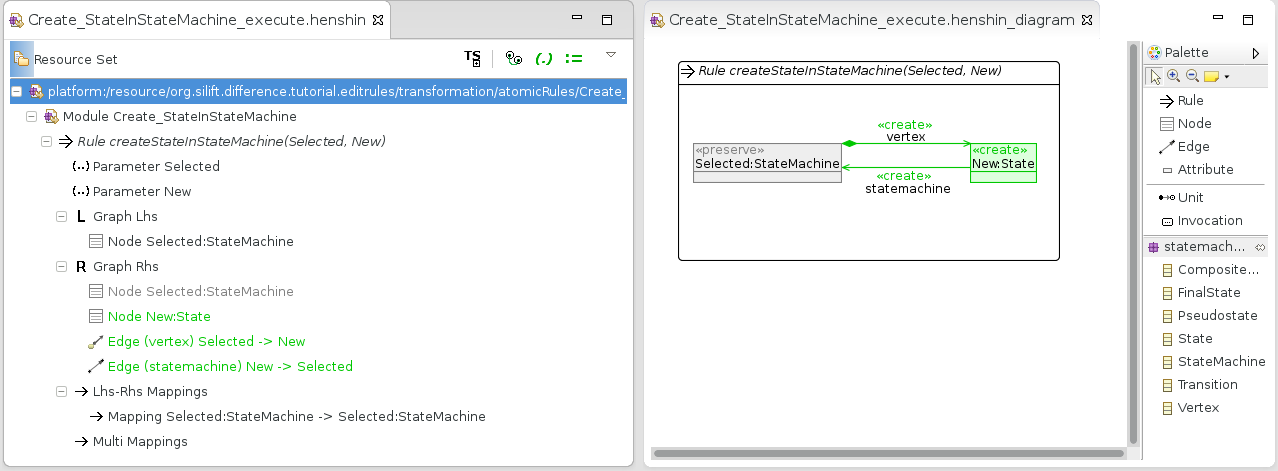
\includegraphics[width=0.8\textwidth]{graphics/silift-editrule_createStateInStateMachine.png}
\caption{Editierregel: createStateInStateMachine}
\label{silift-editrule_createStateInStateMachine}
\end{figure}

Wie bereits erwähnt, verlangt SiLift für jede Editieroperation immer ein Modul mit genau einer Unit und (mit Ausnahme geschachtelter Regeln) einer darin enthaltenen Regel.
Diese Unit muss per Konvention den Namen \textit{mainUnit} tragen.\\
Zwar lassen sich die Units ebenfalls im graphenbasierten Editor erstellen, dennoch ist in unserem Fall der baumbisierte Editor zu bevorzugen.\\
Wechseln Sie in den baumbasierten Editor, indem sie die \texttt{*\_execute.henshin} öffnen.
Im Gegensatz zur graphischen Repräsentation der Regel, lassen sich im baumbasierten Editor die linke und rechte Seite der Transformationsregel genau unterscheiden.
Beim Anwenden einer Regel wird der Arbeitsgraph auf das Vorkommen des Teilgraphen der LHS untersucht. In unserem Beispiel also auf den Teilgraphen, der nur  einen Knoten vom Typ \texttt{StateMachine} enthält.
Durch einen Objekt-Parameter sagen wir zusätzlich um welchen Knoten vom Typ \texttt{StateMachine} es sich genau handeln muss.
Existiert ein solcher Teilgraph, so wird dieser durch den Graphen der RHS ersetzt.
In diesem Fall also einer \texttt{StateMachine}, einem \texttt{State} und den beiden Referenzen \texttt{statemachine} und \texttt{state}.
Zu beachten ist, dass es sich bei dem \texttt{StateMachine}-Knoten um einen "'\textit{preserve}"'-Anteil der Regel handelt, also einem Knoten der eigentlich nicht verändert wird. 
Dazu muss dieser Knoten auf beiden Seiten der Regel vorkommen und ein sogenanntes \textit{Mapping} zwischen diesen existieren (vgl. Abb. \ref{silift-editrule_createStateInStateMachine}: links).\\
Zum Erstellen der mainUnit klicken Sie mit der rechten Maustaste auf \texttt{Module} und wählen \texttt{New Child} $\triangleright$ \texttt{PriorityUnit} (vgl. Abb \ref{silift-editrule_create_priority_unit}).

\begin{figure}[H]
\centering
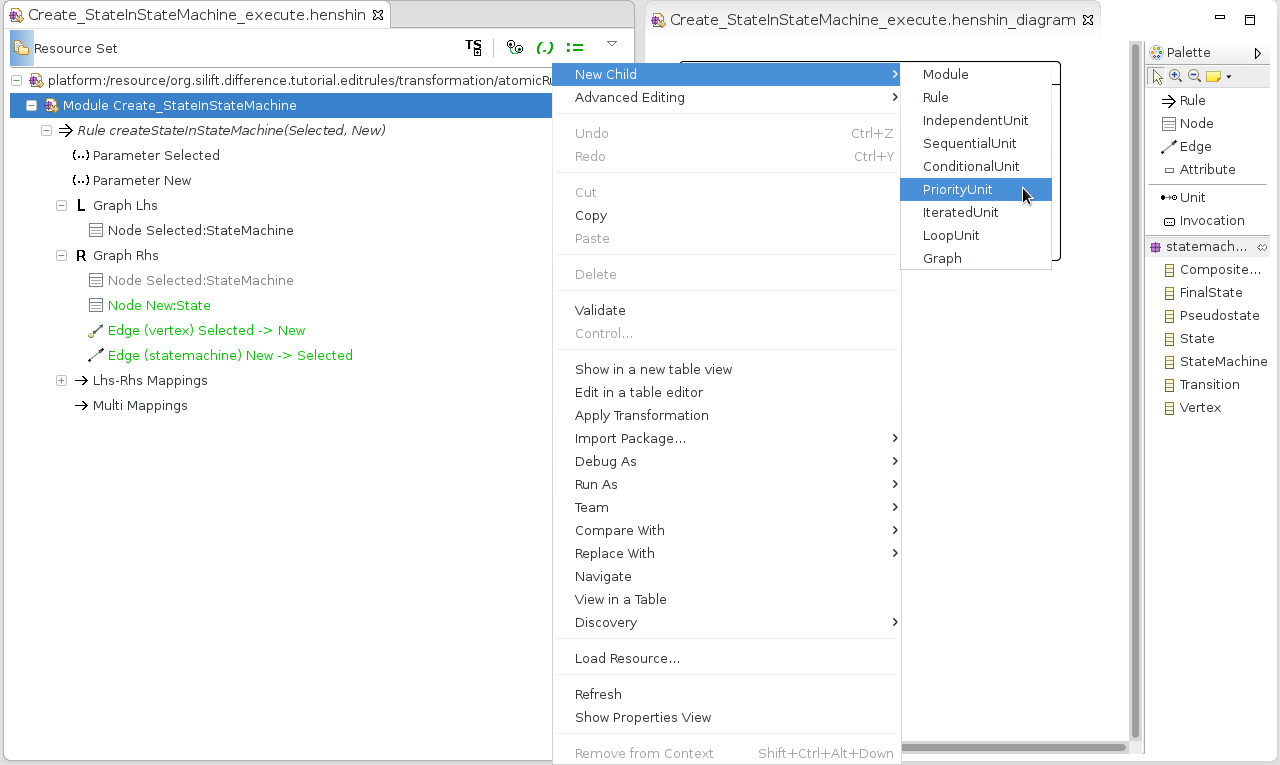
\includegraphics[width=0.8\textwidth]{graphics/silift-editrule_create_priority_unit.png}
\caption{Editierregel: Erstellen einer \textit{Priority Unit}}
\label{silift-editrule_create_priority_unit}
\end{figure}

Nennen Sie diese in "'\textit{mainUnit}"' um und kopieren Sie die eigentliche Regel per \textit{Drag and Drop} in die Unit hinein.\\
Zusätzlich muss die Unit die gleiche Anzahl an Parametern besitzen, wie die Regel. 
Selektieren Sie dazu die \textit{Priority Unit} mit der rechten Maustaste und wählen Sie \texttt{New Child} $\triangleright$ \texttt{Parameter} (vgl. Abb. \ref{silift-editrule_unit_create_parameter}). 
Dabei dürfen die Namen der Parameter durchaus von denen in der Regel abweichen.\\

\textbf{Hinweis}: In Ausnahmefällen kann eine Unit auch weniger Parameter definieren als die beinhaltete Regel. So z.B., wenn die Regel intern Variablen benötigt (z.B. bei der Berechnung von Attributwerten). Derartige interne Variablen werden in Henshin-Regeln auch als Parameter deklariert und sind von Übergabeparametern nicht zu unterscheiden. Die Parameter der Unit repräsentieren letztlich aber die extern sichtbaren Parameter der Editieroperation, also die Signatur der Editieroperation.

\textbf{WICHTIG}: Es muss immer ein \textit{in}-Parameter mit dem Namen \texttt{selectedEObject} existieren, der einen vorhanden Knoten hinein gibt, der zum Kontext der Editierregel gehört.


\begin{figure}[H]
\centering
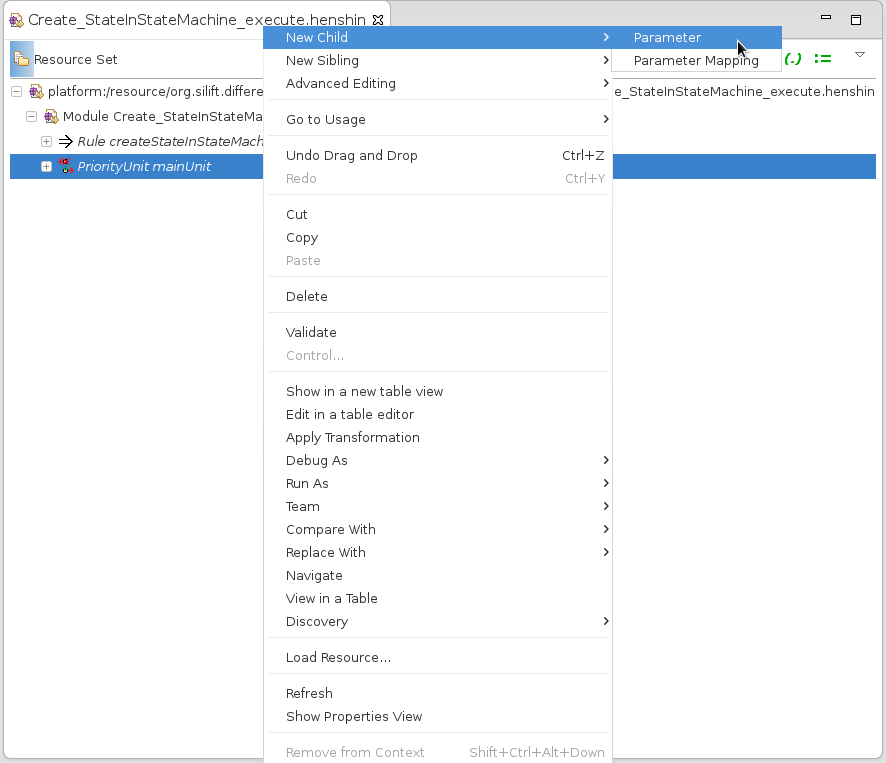
\includegraphics[width=0.6\textwidth]{graphics/silift-editrule_unit_create_parameter.png}
\caption{Editierregel: Erstellen von Parametern}
\label{silift-editrule_unit_create_parameter}
\end{figure}

Nachdem Sie die Parameter erstellt haben müssen diese nun auf die entsprechenden Parameter der Regel "'\textit{gemappt}"' werden.
Durch das \textit{Mapping} wird die Richtung der Parameter (\texttt{in}/\texttt{out}) festgelegt.
Klicken Sie wieder mit der rechten Maustaste auf die \textit{Priority Unit} und wählen Sie diesmal \texttt{New Child} $\triangleright$ \texttt{Parameter Mapping}.\\
Jedes \textit{Parameter-Mapping} besteht aus einem \texttt{Source}- und \texttt{Target}-Parameter, welche unter der \textit{Properties-View} gesetzt werden können.\\

\label{in/out_parameter}
Wird ein Parameter der \textit{Unit} auf einen Parameter der \textit{Rule} gemappt, so handelt es sich um einen \textit{in-Parameter} der aus dem aktuellen Arbeitsgraphen ein Objekt bzw. Knoten an die Regel übergibt (vgl. Abb. \ref{silift-editrule_parametermapping_in}). 
Für \texttt{selectedEObject} ist das immer der Fall. 
Das gleiche gilt für Objekte die gelöscht werden sollen.

\begin{figure}[H]
\centering
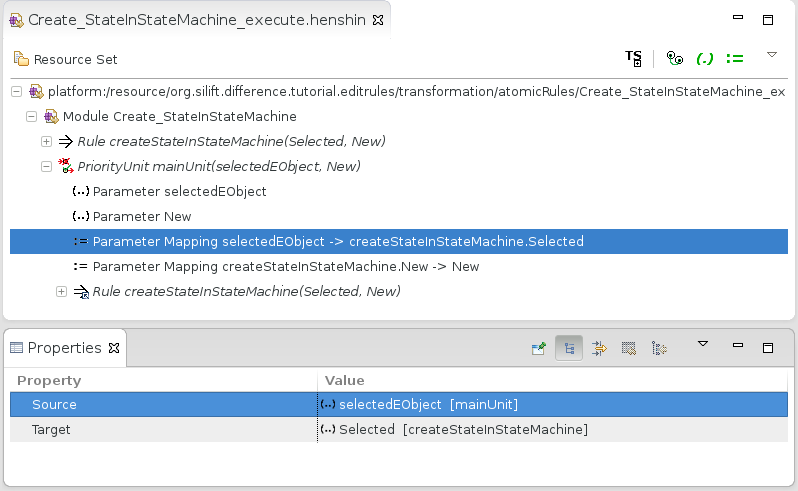
\includegraphics[width=0.6\textwidth]{graphics/silift-editrule_parametermapping_in.png}
\caption{Editierregel: \textit{in-Parameter}}
\label{silift-editrule_parametermapping_in}
\end{figure}

Objekte, welche durch die \textit{Rule} erzeugt werden, müssen durch \textit{out-Parameter}, über die \textit{Unit} zurück an den Arbeitsgraphen gegeben werden.
D.h. der entsprechende Parameter der \textit{Rule} muss auf einen Parameter der \textit{Unit} gemappt werden (vgl. \ref{silift-editrule_parametermapping_out}).
 
\begin{figure}[H]
\centering
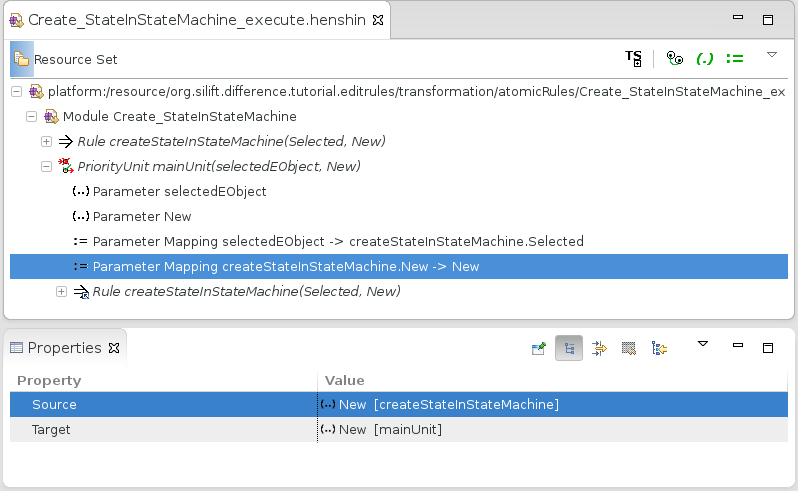
\includegraphics[width=0.6\textwidth]{graphics/silift-editrule_parametermapping_out.png}
\caption{Editierregel: \textit{out-Parameter}}
\label{silift-editrule_parametermapping_out}
\end{figure}

Damit ist die Regel \texttt{createStateInStateMachine} fertig.


\subsubsection*{Delete-Regeln}

Im vorherigem Abschnitt haben Sie gelernt, worauf Sie beim Erstellen einer \textit{Create-Regel} achten müssen.
Neben dem Hinzufügen einzelner Modellelemente, benötigt man jedoch auch Regeln, um Elemente zu verschieben oder aus dem Modell zu entfernen.\\
Erstellen Sie analog zum vorherigem Abschnitt ein neues Henshin-Modell mit dem Namen \texttt{DELETE\_StateInStateMachine\_execute.henshin} und dem entsprechenden Diagramm.
Ersetzen Sie den \textit{"'Stereotypen"'} \texttt{create} durch \texttt{delete} (vgl. Abb \ref{silift-editrule_deleteStateInStateMachine}).

\begin{figure}[H]
\centering
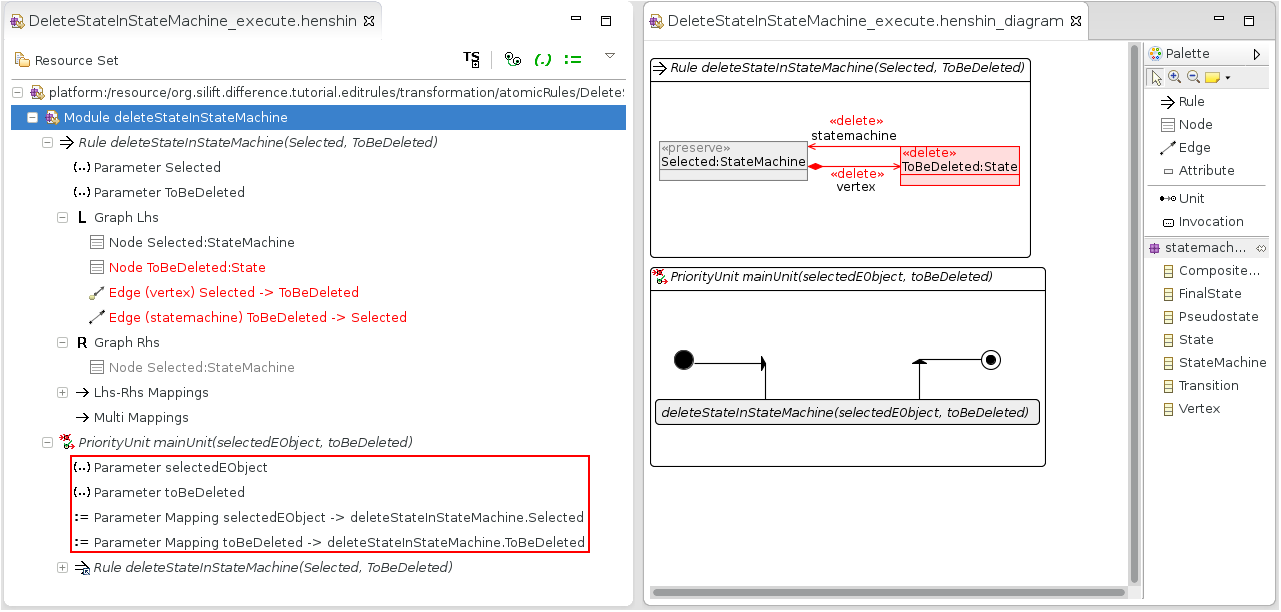
\includegraphics[width=0.8\textwidth]{graphics/silift-editrule_delete_stateInStateMachine.png}
\caption{Editierregel: \texttt{deleteStateInStateMachine}}
\label{silift-editrule_deleteStateInStateMachine}
\end{figure}

Zu beachten ist, dass dieser Regel anstatt einem, zwei Objekte übergeben wird. 
Des Weiteren gibt die Regel auch kein Objekt zurück. 
Dem entsprechend muss das Parameter Mapping angepasst werden (vgl. Abb. \ref{silift-editrule_deleteStateInStateMachine}).\\
Ein weiterer wichtiger Punkt beim Löschen von Elementen sind sogenannte \textit{hängende Referenzen} (engl. \textit{dangling edges}).\\
Abbildung \ref{statemachine_garagedoor} beschreibt die Funktionsweise eines Garagentors in Form eines Zustandsautomaten. 
Initial ist der Zustandsautomat im Zustand \texttt{geschlossen}. 
Bei Tastendruck wird der Zustand \texttt{öffnend} eingenommen usw.

\begin{figure}[H]
\centering
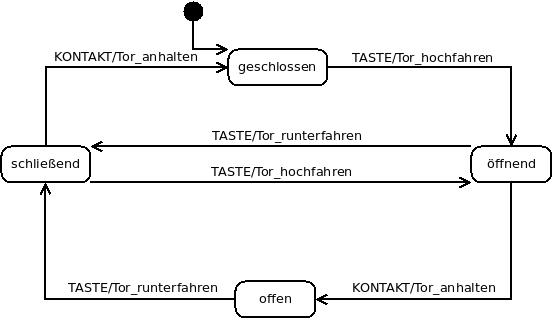
\includegraphics[width=0.5\textwidth]{graphics/statemachine-garagedoor.jpg}
\caption{Zustandsautomat: Garagentor}
\label{statemachine_garagedoor}
\end{figure}

Die interne Repräsentation des Modells, mit der Henshin arbeitet, ist in Abbildung \ref{henshin_workinggraph_garagedoor} zu sehen. 
Um die Übersicht zu behalten wurden, mit Ausnahme der umrandeten Elemente ,einige Referenzen ausgelassen.  

\begin{figure}[H]
\centering
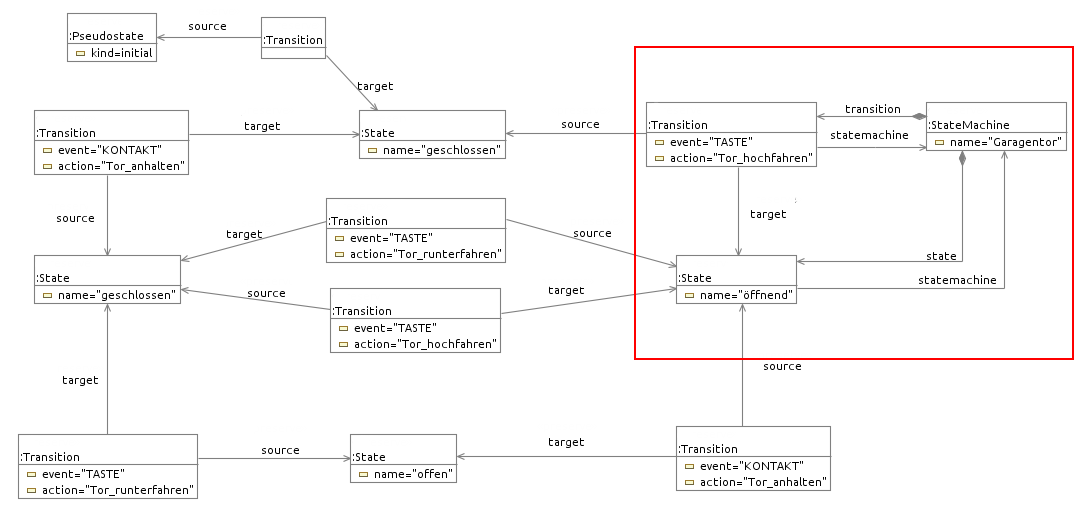
\includegraphics[width=0.8\textwidth]{graphics/henshin-workinggraph_garagedoor.png}
\caption{Arbeitsgraph}
\label{henshin_workinggraph_garagedoor}
\end{figure}

Beim Anwenden der Regel \texttt{deleteSateInStateMachine}, um z.B. den Zustand \texttt{öffnend} zu löschen, würden hängende Referenzen und somit ein inkonsistentes Modell entstehen. Die Regel löscht nur die Referenzen zwischen \textit{StateMachine} und \textit{State}, alle anderen bleiben bestehen (vgl. Abb. \ref{henshin_workinggraph_garagedoor_danglingEdges}). 

\begin{figure}[H]
\centering
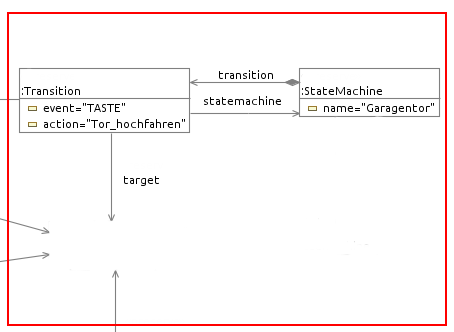
\includegraphics[width=0.5\textwidth]{graphics/henshin-workinggraph_garagedoor_danglingEdges.png}
\caption{hängende Referenzen}
\label{henshin_workinggraph_garagedoor_danglingEdges}
\end{figure}

Um in so einem Fall das Anwenden einer Regel zu verhindern, muss für die entsprechende Regel die Option \texttt{Check Dangling} auf \texttt{true} gesetzt sein (vgl. \ref{silift-silift-editrule_delete_stateInStateMachine_checkDangling}).\\

\textbf{Hinweis}: Die Option \texttt{Check Dangling} ist per \textit{default} auf \texttt{true} gesetzt und sollte bei der Verwendung von \textit{SiLift} auch nicht geändert werden.


\begin{figure}[H]
\centering
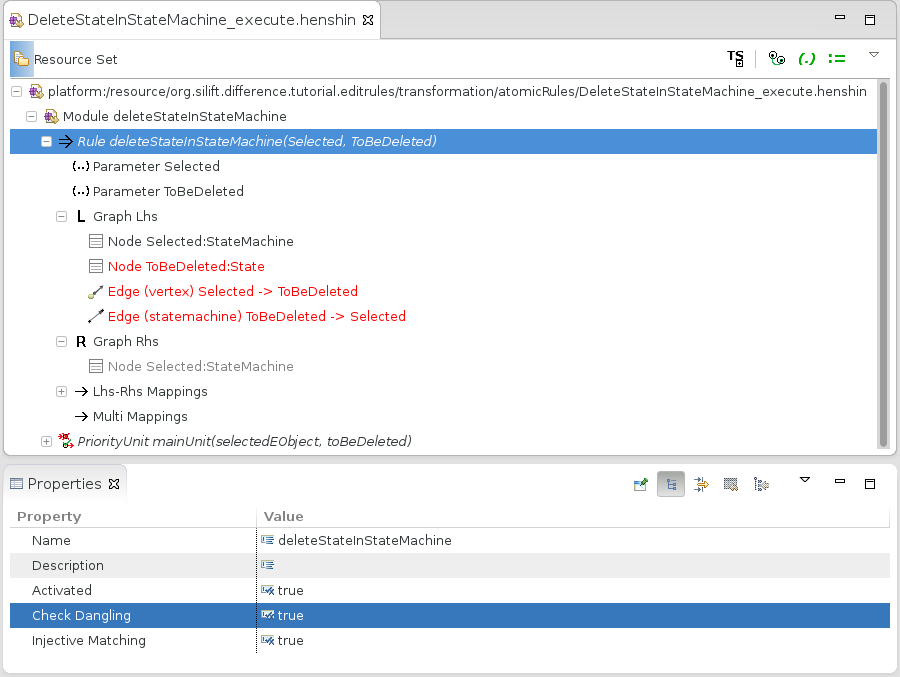
\includegraphics[width=0.6\textwidth]{graphics/silift-editrule_delete_stateInStateMachine_checkDangling.png}
\caption{hängende Referenzen}
\label{silift-silift-editrule_delete_stateInStateMachine_checkDangling}
\end{figure}


\subsubsection*{Negative Application Conditions}

Abbildung \ref{silift-editrule_create_transitionFromInitialToState} zeigt eine Editierregel, die eine neue Transition von einem Startzustand zu einem normalen Zustand erzeugt.

\begin{figure}[H]
\centering
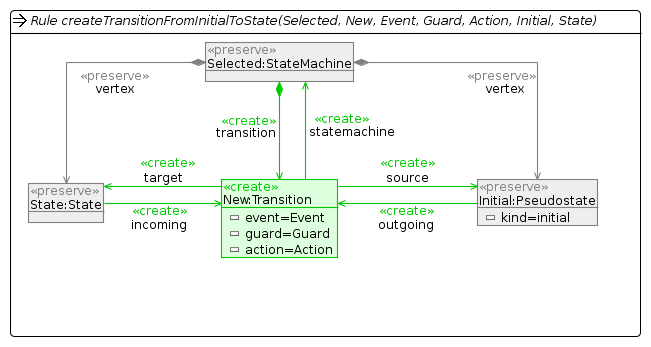
\includegraphics[width=0.6\textwidth]{graphics/silift-editrule_create_transitionFromInitialToState.png}
\caption{Editierregel: \texttt{createTransitionFromInitialToState}}
\label{silift-editrule_create_transitionFromInitialToState}
\end{figure}

Betrachtet man jetzt nochmal das Metamodell  auf Seite \pageref{subsec:metamodel}, so darf ein \textit{Startzustand} maxi\-mal eine ausgehende Transition besitzen.
Solche Bedingungen können mit \textit{NACs} umgesetzt werden.
Dazu modelliert man den unerwünschten Fall als Teilgraph und markiert diesen mit dem \textit{"'Stereotyp"'} \texttt{forbid} (vgl. Abb. \ref{silift-editrule_create_transitionFromInitialToState_with_forbid}).

\begin{figure}[H]
\centering
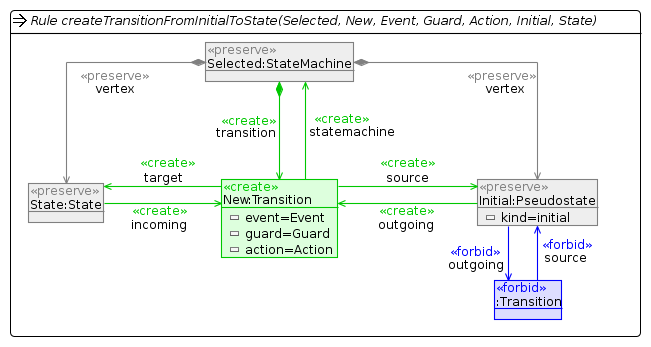
\includegraphics[width=0.6\textwidth]{graphics/silift-editrule_create_transitionFromInitialToState_with_forbid.png}
\caption{Editierregel: \texttt{createTransitionFromInitialToState} mit \textit{NAC}}
\label{silift-editrule_create_transitionFromInitialToState_with_forbid}
\end{figure}

Dieser erzeugt in der \textit{LHS} eine \texttt{Application Condition}, welche negiert wird.
Die Condition besitzt ein Graph-Objekt, welches den unerwünschten Teilgraphen modelliert.\\
In unserem Fall besteht der Teilgraph aus vier Knoten und vier Kante.
Zusätzlich wird noch ein Mapping der Knoten \texttt{Initial:Pseudostate}, \texttt{Selected:StateMachine} und \texttt{State:State} aus der LHS auf den NAC-Graphen benötigt (vgl. Abb. \ref{silift-editrule_create_transitionFromInitialToState_with_forbid}).


\begin{figure}[H]
\centering
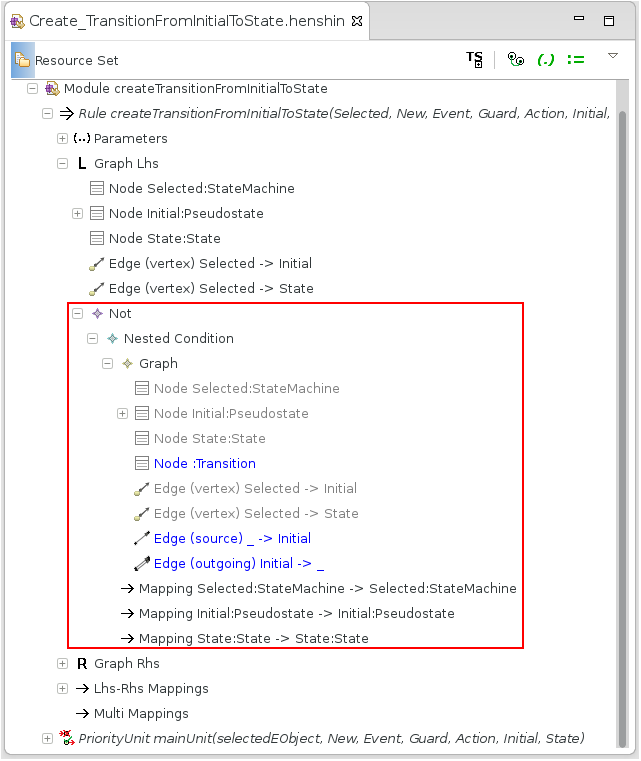
\includegraphics[width=0.5\textwidth]{graphics/silift-editrule_create_transitionFromInitialToState_with_forbid_treeView.png}
\caption{Editierregel: \texttt{createTransitionFromInitialToState} mit \textit{NAC}}
\label{silift-editrule_create_transitionFromInitialToState_with_forbid_treeView}
\end{figure}

\textbf{Hinweis}: In Henshin lassen sich \textit{NACs} beliebig schachteln und durch boolsche Operatoren wie \texttt{AND} und \texttt{OR} verknüpfen. \textit{SiLift} unterstützt in der aktuellen Version nur die Konjunktion von Anwendungsbedingungen.


\section{Generieren von Erkennungsregeln}

Um einer \textit{low-level} Änderung der technischen Differenz eine bestimmte Editieroperation zuzuordnen werden sogenannte \textit{Erkennungsregeln} benötigt. 
Dabei handelt es sich ebenfalls um Henshin-Regeln, die sich mit Hilfe des \textit{Recognitionrule Generators} direkt aus den zuvor erstellten Editierregeln ableiten lassen.


\subsection{Rulebase Plug-in Projekt}

Um ein Rulebase Plug-in Projekt zu erstellen importieren sie am besten ein bestehendes Rulebase Plug-in Projekt (z.B. \texttt{org.sidiff.ecore.recognitionrules.atomic}): File $\triangleright$ Import $\triangleright$ Plug-Ins and Fragments $\triangleright$ Projects with source folders.\\
Anschließend passen Sie den Projektnamen und weitere projektspezifische Bezeichner an Ihre Bedürfnisse an. Exisitierende Rulebases können Sie aus dem Projekt löschen. Verfahren Sie anschließend gemäß Abschnitt \ref{sec:rbfile} mit dem eigentlichen Erzeugen der neuen Erkennungsregeln und des sog. Rulebase-Files.\\

\textbf{Hinweis}: In Kürze wird für das Erstellen eines Rulebase Plug-in Projekts auch ein komfortablerer Wizard zur Verfügung stehen.

% TODO: Wieder einbinden und nochmals prüfen, sobald Bug in RB-Projekt Wizard gefixed.
%
% Gehen Sie auf \texttt{File} $\triangleright$ \texttt{New} $\triangleright$ \texttt{Other...} und wählen Sie \texttt{SiLift} $\triangleright$ \texttt{Rulebase Plug-in Project} aus (vgl. Abb. \ref{silift-wizard_rulebase_page01}).
% 
% \begin{figure}[H]
% \centering
% 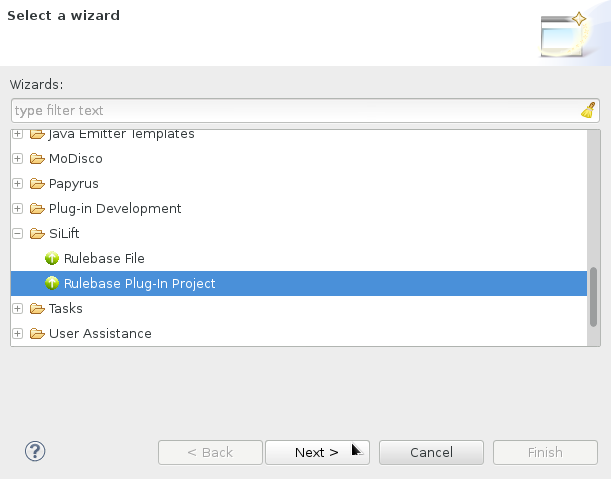
\includegraphics[width=0.5\textwidth]{graphics/silift-wizard_rulebase_page01.png}
% \caption{Erstellen eines \textit{Rulebase Plug-in Projects}}
% \label{silift-wizard_rulebase_page01}
% \end{figure}
% 
% Klicken Sie auf \texttt{Next} und geben Sie einen Projektnamen ein (vgl. Abb. \ref{silift-wizard_rulebase_page02}).
% 
% \begin{figure}[H]
% \centering
% 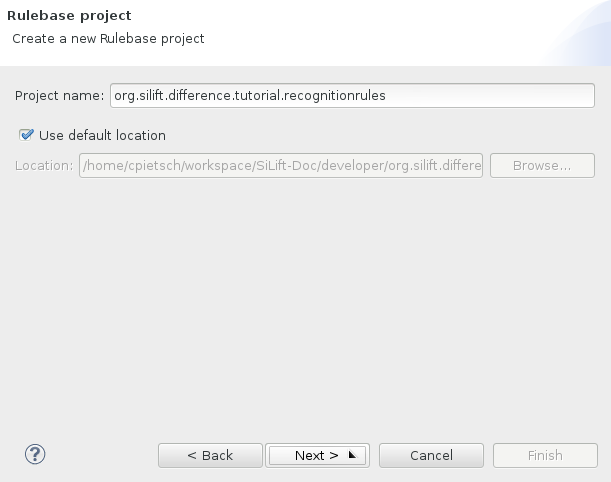
\includegraphics[width=0.5\textwidth]{graphics/silift-wizard_rulebase_page02.png}
% \caption{Erstellen eines \textit{Rulebase Plug-in Projects}}
% \label{silift-wizard_rulebase_page02}
% \end{figure}
% 
% Danach müssen noch die Editierregeln ausgewählt und unter einem entsprechenden Namen abgespeichert werden (vgl. Abb. \ref{silift-wizard_rulebase_page03}).
% SiLift erzeugt nun die Erkennungsregeln und speichert diese in einer \textit{Rulebase}.
% 
% \begin{figure}[H]
% \centering
% 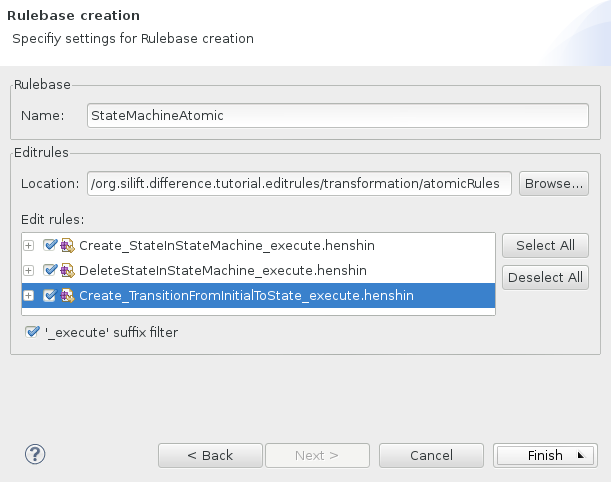
\includegraphics[width=0.5\textwidth]{graphics/silift-wizard_rulebase_page03.png}
% \caption{Erstellen eines \textit{Rulebase Plug-in Projects}}
% \label{silift-wizard_rulebase_page03}
% \end{figure}




\subsection{Rulebase File}
\label{sec:rbfile}

Des Weiteren kann es sein, dass Sie für eine Domain (hier unser Zustandsautomat) mehrere Regelbasen zur Verfügung stellen möchten.
Das ist z.B. dann der Fall, wenn man sich die Editierregeln mittels Generator hat generieren lassen und einige jetzt noch manuell nachgebessert oder ergänzt werden müssen.
Um eine neue Regelbasis zu erstellen, gehen Sie wieder auf \texttt{File} $\triangleright$ \texttt{New} $\triangleright$ \texttt{Other...} und wählen Sie  \texttt{SiLift} $\triangleright$ \texttt{Rulebase File}

\begin{figure}[H]
\centering
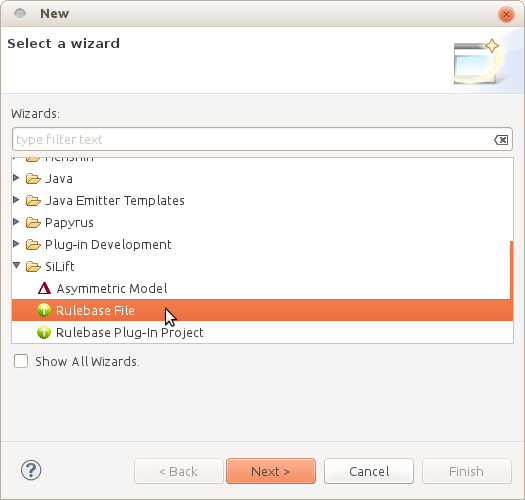
\includegraphics[width=0.5\textwidth]{graphics/silift-rulebase_file1.png}
\caption{Erstellen einer neuen Regelbasis}
\label{silift_rulebase_file1}
\end{figure}

Im nächsten Schritt wählen Sie das Verzeichnis \texttt{rulebase} des bestehenden Projekts für die Erkennungsregeln und geben der Regelbasis einen Namen (vgl. Abb. \ref{silift_rulebase_file2}).

\begin{figure}[H]
\centering
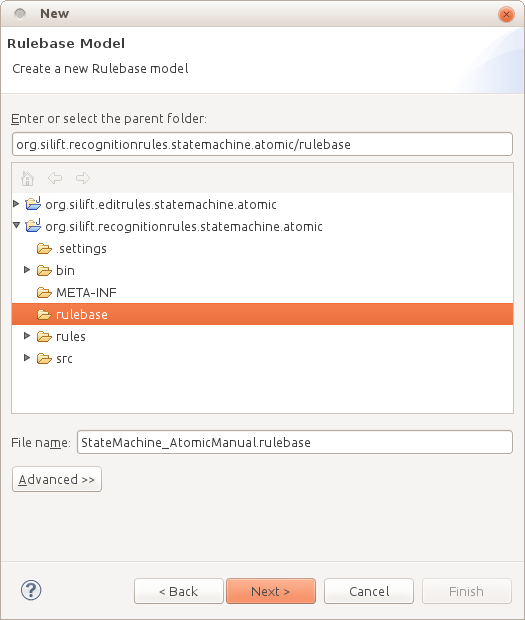
\includegraphics[width=0.5\textwidth]{graphics/silift-rulebase_file2.png}
\caption{Erstellen einer neuen Regelbasis}
\label{silift_rulebase_file2}
\end{figure}

Jetzt wählen Sie wie bereits zuvor die gewünschten Editierregeln aus und klicken auf \texttt{Finish} (vgl. Abb. \ref{silift_rulebase_file3}).

\begin{figure}[H]
\centering
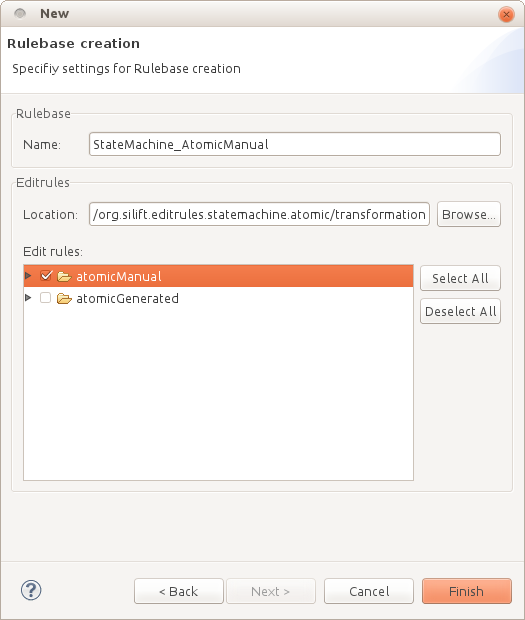
\includegraphics[width=0.5\textwidth]{graphics/silift-rulebase_file3.png}
\caption{Erstellen einer neuen Regelbasis}
\label{silift_rulebase_file3}
\end{figure}

Damit haben Sie Ihrem Projekt eine neue Regelbasis hinzugefügt (vgl. Abb. \ref{silift_RR_Project_Explorer}).
Als nächstes muss sich diese Regelbasis noch als Erweiterung (engl. \textit{Extension}) bei dem Plugin registrieren.


\begin{figure}[H]
\centering
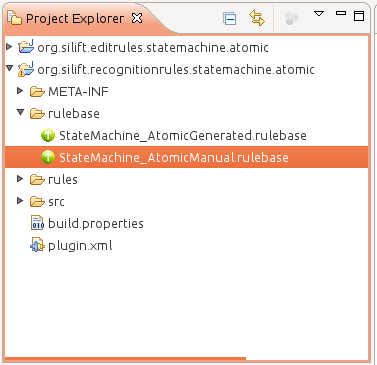
\includegraphics[width=0.3\textwidth]{graphics/silift-RR_Project_Explorer.png}
\caption{Project Explorer: Regelbasen}
\label{silift_RR_Project_Explorer}
\end{figure}

Öffnen Sie das Verzeichnis \texttt{src} über den \textit{Package Explorer}, kopieren Sie die bereits existierende Klasse und nennen diese entsprechend um (vgl. Abb. \ref{silift_Extension_RuleBase}).
Danach öffnen Sie die Klasse und passen den Wert der Variablen \texttt{RULE\_BASE\_NAME} entsprechend an. 

\begin{figure}[H]
\centering
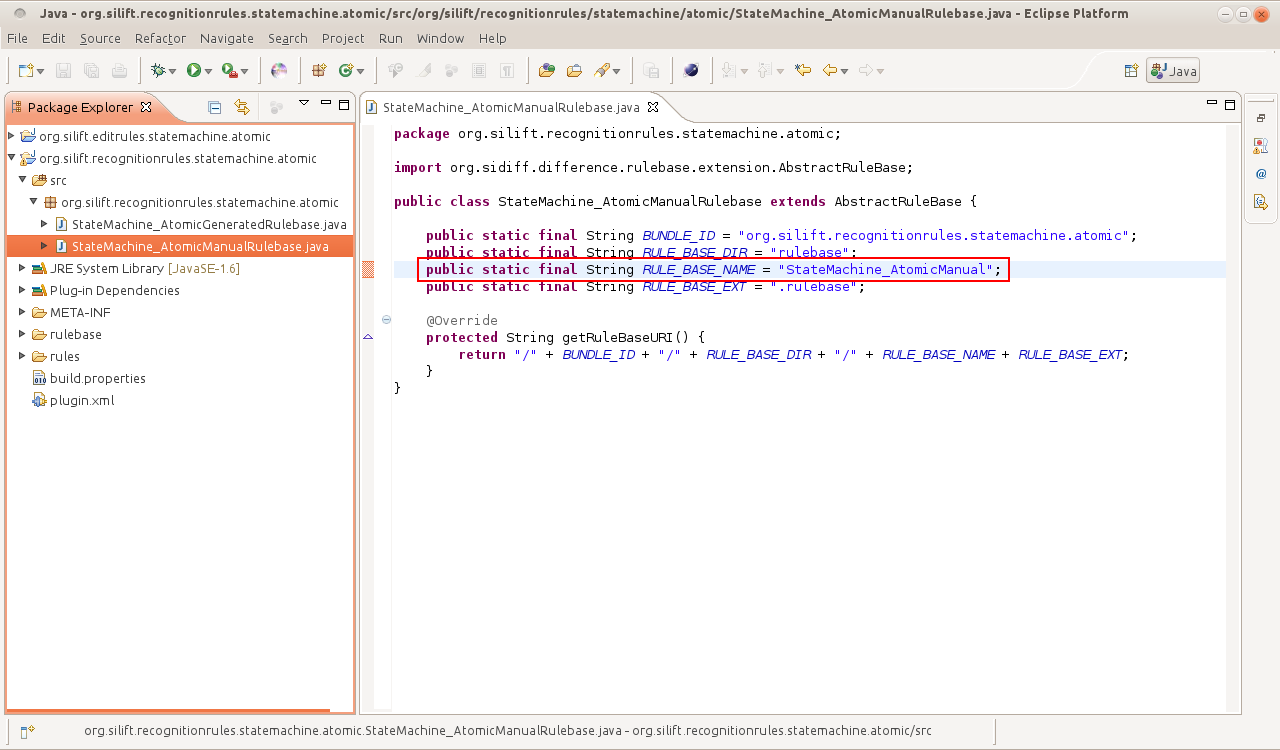
\includegraphics[width=0.8\textwidth]{graphics/silift-Extension_RuleBase.png}
\caption{Klasse: StateMachine\_AtomicManualRulebase}
\label{silift_Extension_RuleBase}
\end{figure}

Öffnen Sie die \texttt{MANIFEST.MF} und wählen Sie den Reiter \texttt{Extensions} aus (vgl. Abb. \ref{silift_Manifest_Extensions}). 


\begin{figure}[H]
\centering
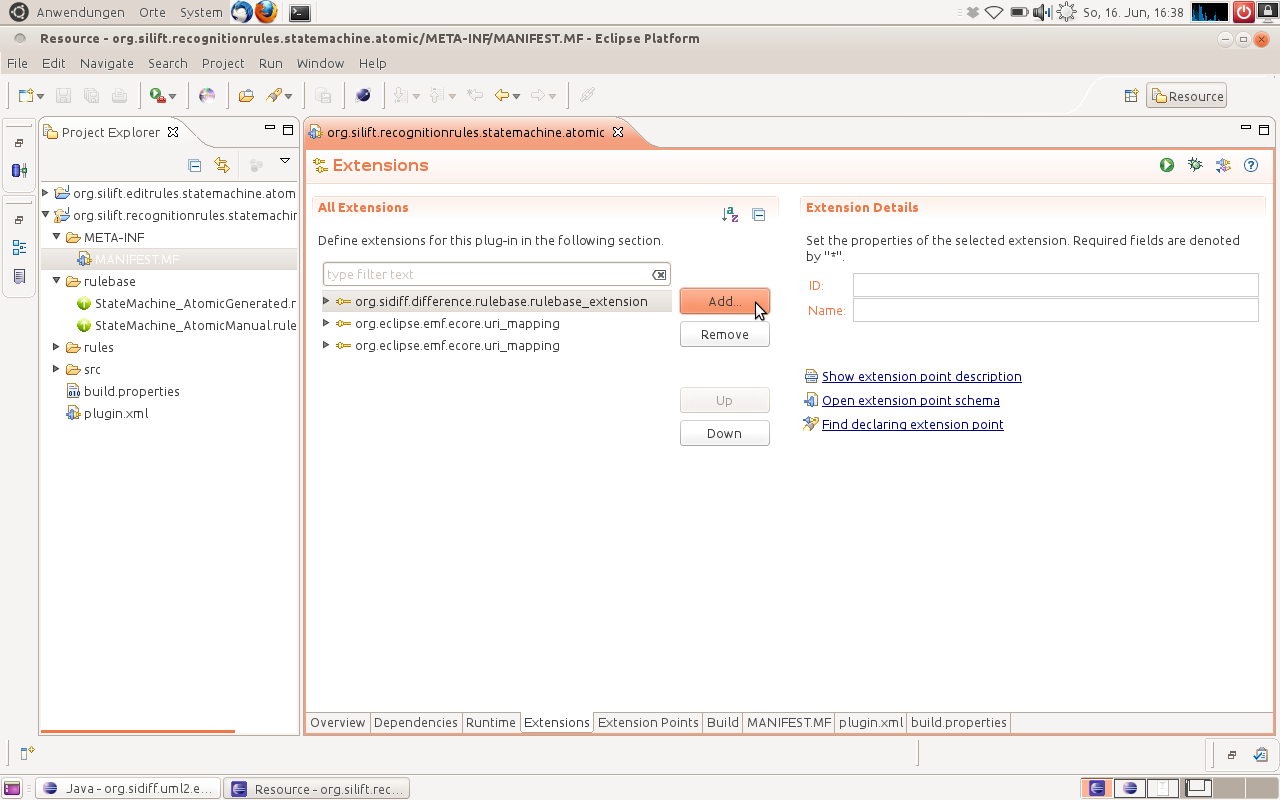
\includegraphics[width=0.8\textwidth]{graphics/silift-Manifest_Extensions.png}
\caption{Manifest.MF: \texttt{Extensions}}
\label{silift_Manifest_Extensions}
\end{figure}


Klicken Sie auf \texttt{Add...} und selektieren Sie den \textit{Extension Point} \texttt{org"".sidiff"".difference"".rulebase"".rulebase""\_extension} (vgl. Abb. \ref{silift_Manifest_Extension_Point}). Klicken Sie auf \texttt{Finish}.

\begin{figure}[H]
\centering
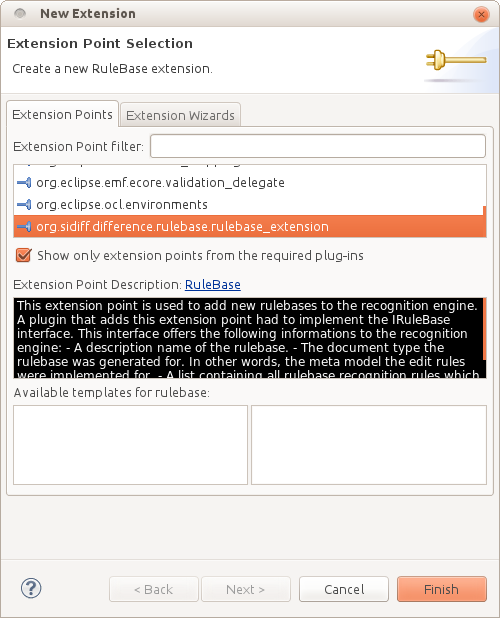
\includegraphics[width=0.5\textwidth]{graphics/silift-Manifest_Extension_Point.png}
\caption{Extension Point: Rule Base}
\label{silift_Manifest_Extension_Point}
\end{figure}


Wechseln Sie danach in den Reiter \texttt{plugin.xml} und fügen dem eben erstellen Extension Point die entsprechende URI der Erweiterung bei (vgl. Abb. \ref{silift_Manifest_plugin}).

\begin{figure}[H]
\centering
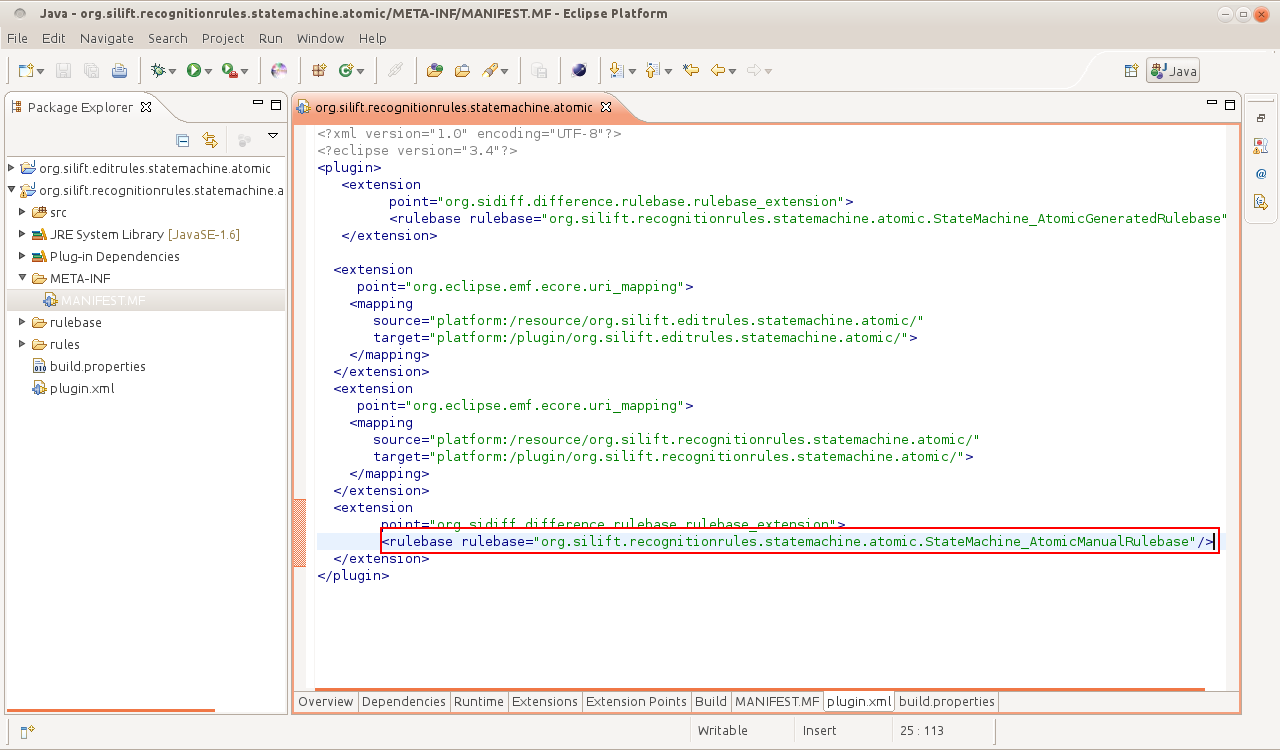
\includegraphics[width=0.8\textwidth]{graphics/silift-Manifest_plugin.png}
\caption{Manifest.MF: \texttt{plugin.xml}}
\label{silift_Manifest_plugin}
\end{figure}



\subsection{Der Rulebase-Manager}
\label{sec:rbmanager}

Generierte Erkennungsregeln können mit Hilfe des \textit{Rulebase Manager} verwaltet werden (vgl. Abb. \ref{silif_Rulebase_Manager}).

\begin{figure}[H]
\centering
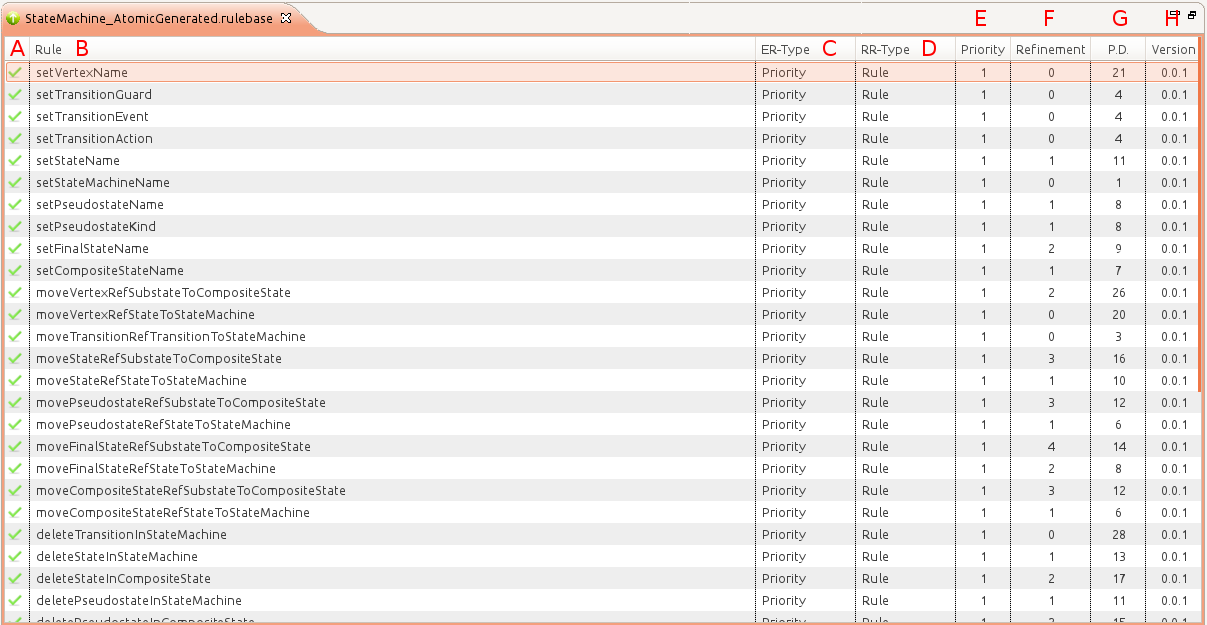
\includegraphics[width=0.8\textwidth]{graphics/silift-Rulebase_Manager.png}
\caption{Erstellen eines \textit{Rulebase Manager}}
\label{silif_Rulebase_Manager}
\end{figure}

\begin{enumerate}[(A)]
\item Durch Klicken auf das Häkchen können einzelne Erkennungsregeln für die \textit{Recognition-Engine} aktiviert (grün) bzw. deaktiviert (grau) werden.

\item Repräsentiert den Verwaltungsname der Editier-, bzw. Erkennungsregel. Dieser kann durch den Rulebase Manager editiert werden, wird aber nur zur Anzeige in der GUI verwendet.

\item Henshin Typ der \textit{mainUnit} der Editierregel (\texttt{Independent}, \texttt{Priority}, \texttt{Sequential} oder \texttt{Amalgamation Unit}).

\item Henshin Typ der Erkennungsregel mainUnit.

\item Priorität der Erkennungsregel:
 Gerade unter zusätzlicher Verwendung komplexer Editierregeln kann es vorkommen, dass zwei \textit{Semantic Change Sets} (vgl. \pageref{page:semantic_change_sets}) die gleichen \textit{low-level}-Änderungen beinhalten. 
Für den Fall kann man einer Regel eine höhere Priorität zuordnen. 

\item \textit{Refinement-Level}: 
Für den Fall, dass auch die Prioritäten zweier identischer \textit{Semantic Change Sets} gleich sind, versucht \textit{SiLift} anhand der Anzahl der Supertypen die "'speziellere"' Regel zu bestimmen. 
D.h. je mehr Supertypen die Knoten der Regel besitzen, desto spezieller ist diese. 

\item \textit{Potential Dependicies}: 
Anzahl der potentiellen Abhängigkeiten zu anderen Editieroperationen. 
Das sequentielle Ausführen mehrere Editieroperationen ist nicht kommutativ, d.h. es können zwischen den jeweiligen Editieroperationen Abhängigkeiten existieren, die beim generieren eines Patches berücksichtigt werden müssen. 

\item Version des verwendeten \textit{Recognitionrule-Generators}.
\end{enumerate}

I.d.R. wächst eine Regelbasis mit der Zeit. 
Es ist so gut wie unmöglich alle möglichen Editieroperationen im Vorfeld aufzudecken und zu implementieren. 
Um Ihrer bestehenden Regelbasis neue Regeln hinzuzufügen klicken Sie auf \texttt{Generate new recognition rules} (vgl. Abb. \ref{silift_generate_new_recognition_rules}) und wählen die entsprechenden Editierregeln aus. 
Die abgeleiteten Erkennungsregeln werden nun der bestehenden Regelbasis hinzugefügt.

\begin{figure}[H]
\centering
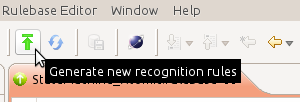
\includegraphics[width=0.25\textwidth]{graphics/silift-generate_new_recognition_rules.png}
\caption{Erkennungsregeln einer bestehenden \textit{Rulebase} hinzufügen}
\label{silift_generate_new_recognition_rules}
\end{figure}


\subsection{Erkennungsregeln deployen und nutzen}
\label{sec:deploying_recognitionrules}

Um die Erkennungsregeln zu testen, gibt es zwei Möglichkeiten:

\begin{enumerate}

\item Eclipse Application: 
Öffnen Sie die \texttt{MANIFEST.MF} des Projekts der Erkennungsregeln und starten sie über das \textit{Launch Icon} (vgl. Abb. \ref{eclipse_run_eclipse_application}) eine zweite Eclipse-Instanz. Innerhalb dieser Instanz sind alle Projekte aus Ihrem Workspace registriert und können verwendet werden.

\begin{figure}[H]
\centering
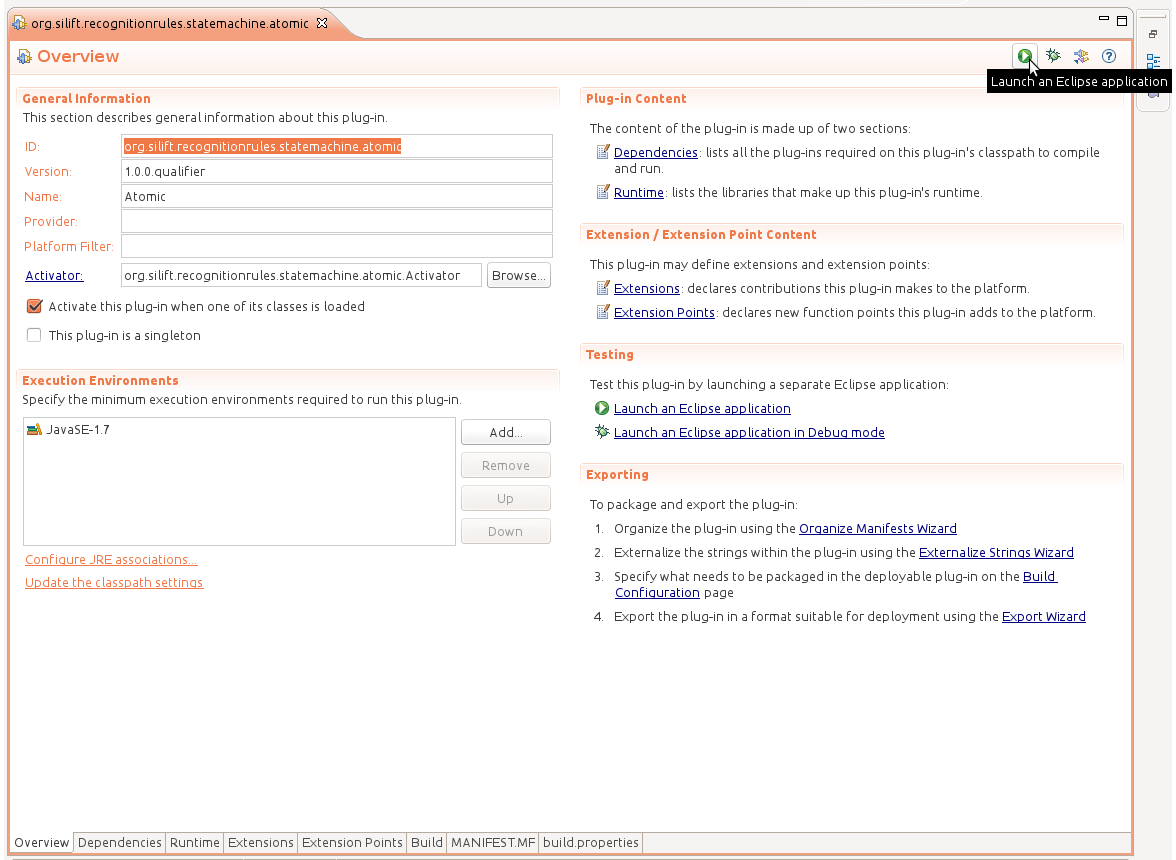
\includegraphics[width=0.8\textwidth]{graphics/eclipse-run_eclipse_application.png}
\caption{Run Ecplipse Application}
\label{eclipse_run_eclipse_application}
\end{figure}


\item Deployable Plugins and Fragments: analog zu Abschnitt \ref{sec:own_matching_engine}.

%Gehen Sie auf \texttt{File} $\triangleright$ \texttt{Export...} um ein Plugin zu "'\textit{deployen}"' (vgl. Abb. \ref{eclipse_export_plugins}).

%\begin{figure}[H]
%\centering
%\includegraphics[width=0.5\textwidth]{graphics/eclipse-export_plugins.png}
%\caption{Plugin exportieren}
%\label{eclipse_export_plugins}
%\end{figure}

%Wählen Sie dann \texttt{Plug-in Development} $\triangleright$ \texttt{Deployable Plugins and Fragments} (vgl. Abb. \ref{eclipse_deployable_plugins_and_fragments1}).

%\begin{figure}[H]
%\centering
%\includegraphics[width=0.5\textwidth]{graphics/eclipse-deployable_plugins_and_fragments1.png}
%\caption{Eclipse - Deployable Plugins and Fragments}
%\label{eclipse_deployable_plugins_and_fragments1}
%\end{figure}

%Selektieren Sie die entsprechenden Plugins und geben Sie als Ort den \texttt{dropins}-Ordner Ihres Eclipses an (vgl. Abb. \ref{eclipse_deployable_plugins_and_fragments2}).
%\vspace{10mm}

%\begin{small}
%\textbf{WICHTIG}: Es müssen sowohl die Erkennungsregeln als auch die Editierregeln selektiert werden.
%\end{small}
%\vspace{5mm}

%\begin{figure}[H]
%\centering
%\includegraphics[width=0.5\textwidth]{graphics/eclipse-deployable_plugins_and_fragments2.png}
%\caption{Eclipse - Deployable Plugins and Fragments}
%\label{eclipse_deployable_plugins_and_fragments2}
%\end{figure}

%Beim nächsten Start von Eclipse werden die erstellten Plugins automatisch registriert und können dann benutzt werden.

\end{enumerate}

Wenn Sie Ihre Regeln erstmal nur testen möchten, ist die erste Variante zu bevorzugen. 
Sofern Sie die zweite Variante nutzen und ggf. mit Hilfe des \textit{Rulebase-Managers} an den Erkennungsregeln  etwas verändern möchten, müssen Sie die installierten Plugins zuerst deinstallieren.\\
Eine umfassende Einführung in die Nutzung von SiLift als Differenzwerkzeug finden Sie im \textbf{SiLift - Benutzerhandbuch für Endanwender}.


\begin{center}
\textbf{ENDE}
\end{center}

\newpage

\section{Links und weitere Informationen}

\begin{itemize}
\item \textbf{EMF-Compare}: \url{http://www.eclipse.org/emf/compare}
\item \textbf{EMF-Henshin}: \url{http://www.eclipse.org/henshin/}
\item \textbf{SERGe:} \url{http://pi.informatik.uni-siegen.de/Projekte/SERGe.php}
\item \textbf{SiDiff}: \url{http://pi.informatik.uni-siegen.de/Projekte/sidiff/}
\item \textbf{SiLift}: \url{http://pi.informatik.uni-siegen.de/Projekte/SiLift/}
\end{itemize} 
\end{document}